\chapter{Predictive Robust Estimation}
\label{ch:probe}
\epigraph{Information is the resolution of uncertainty.}{Claude Shannon}

\section{Introduction}

\begin{figure*}[h!]
\centering
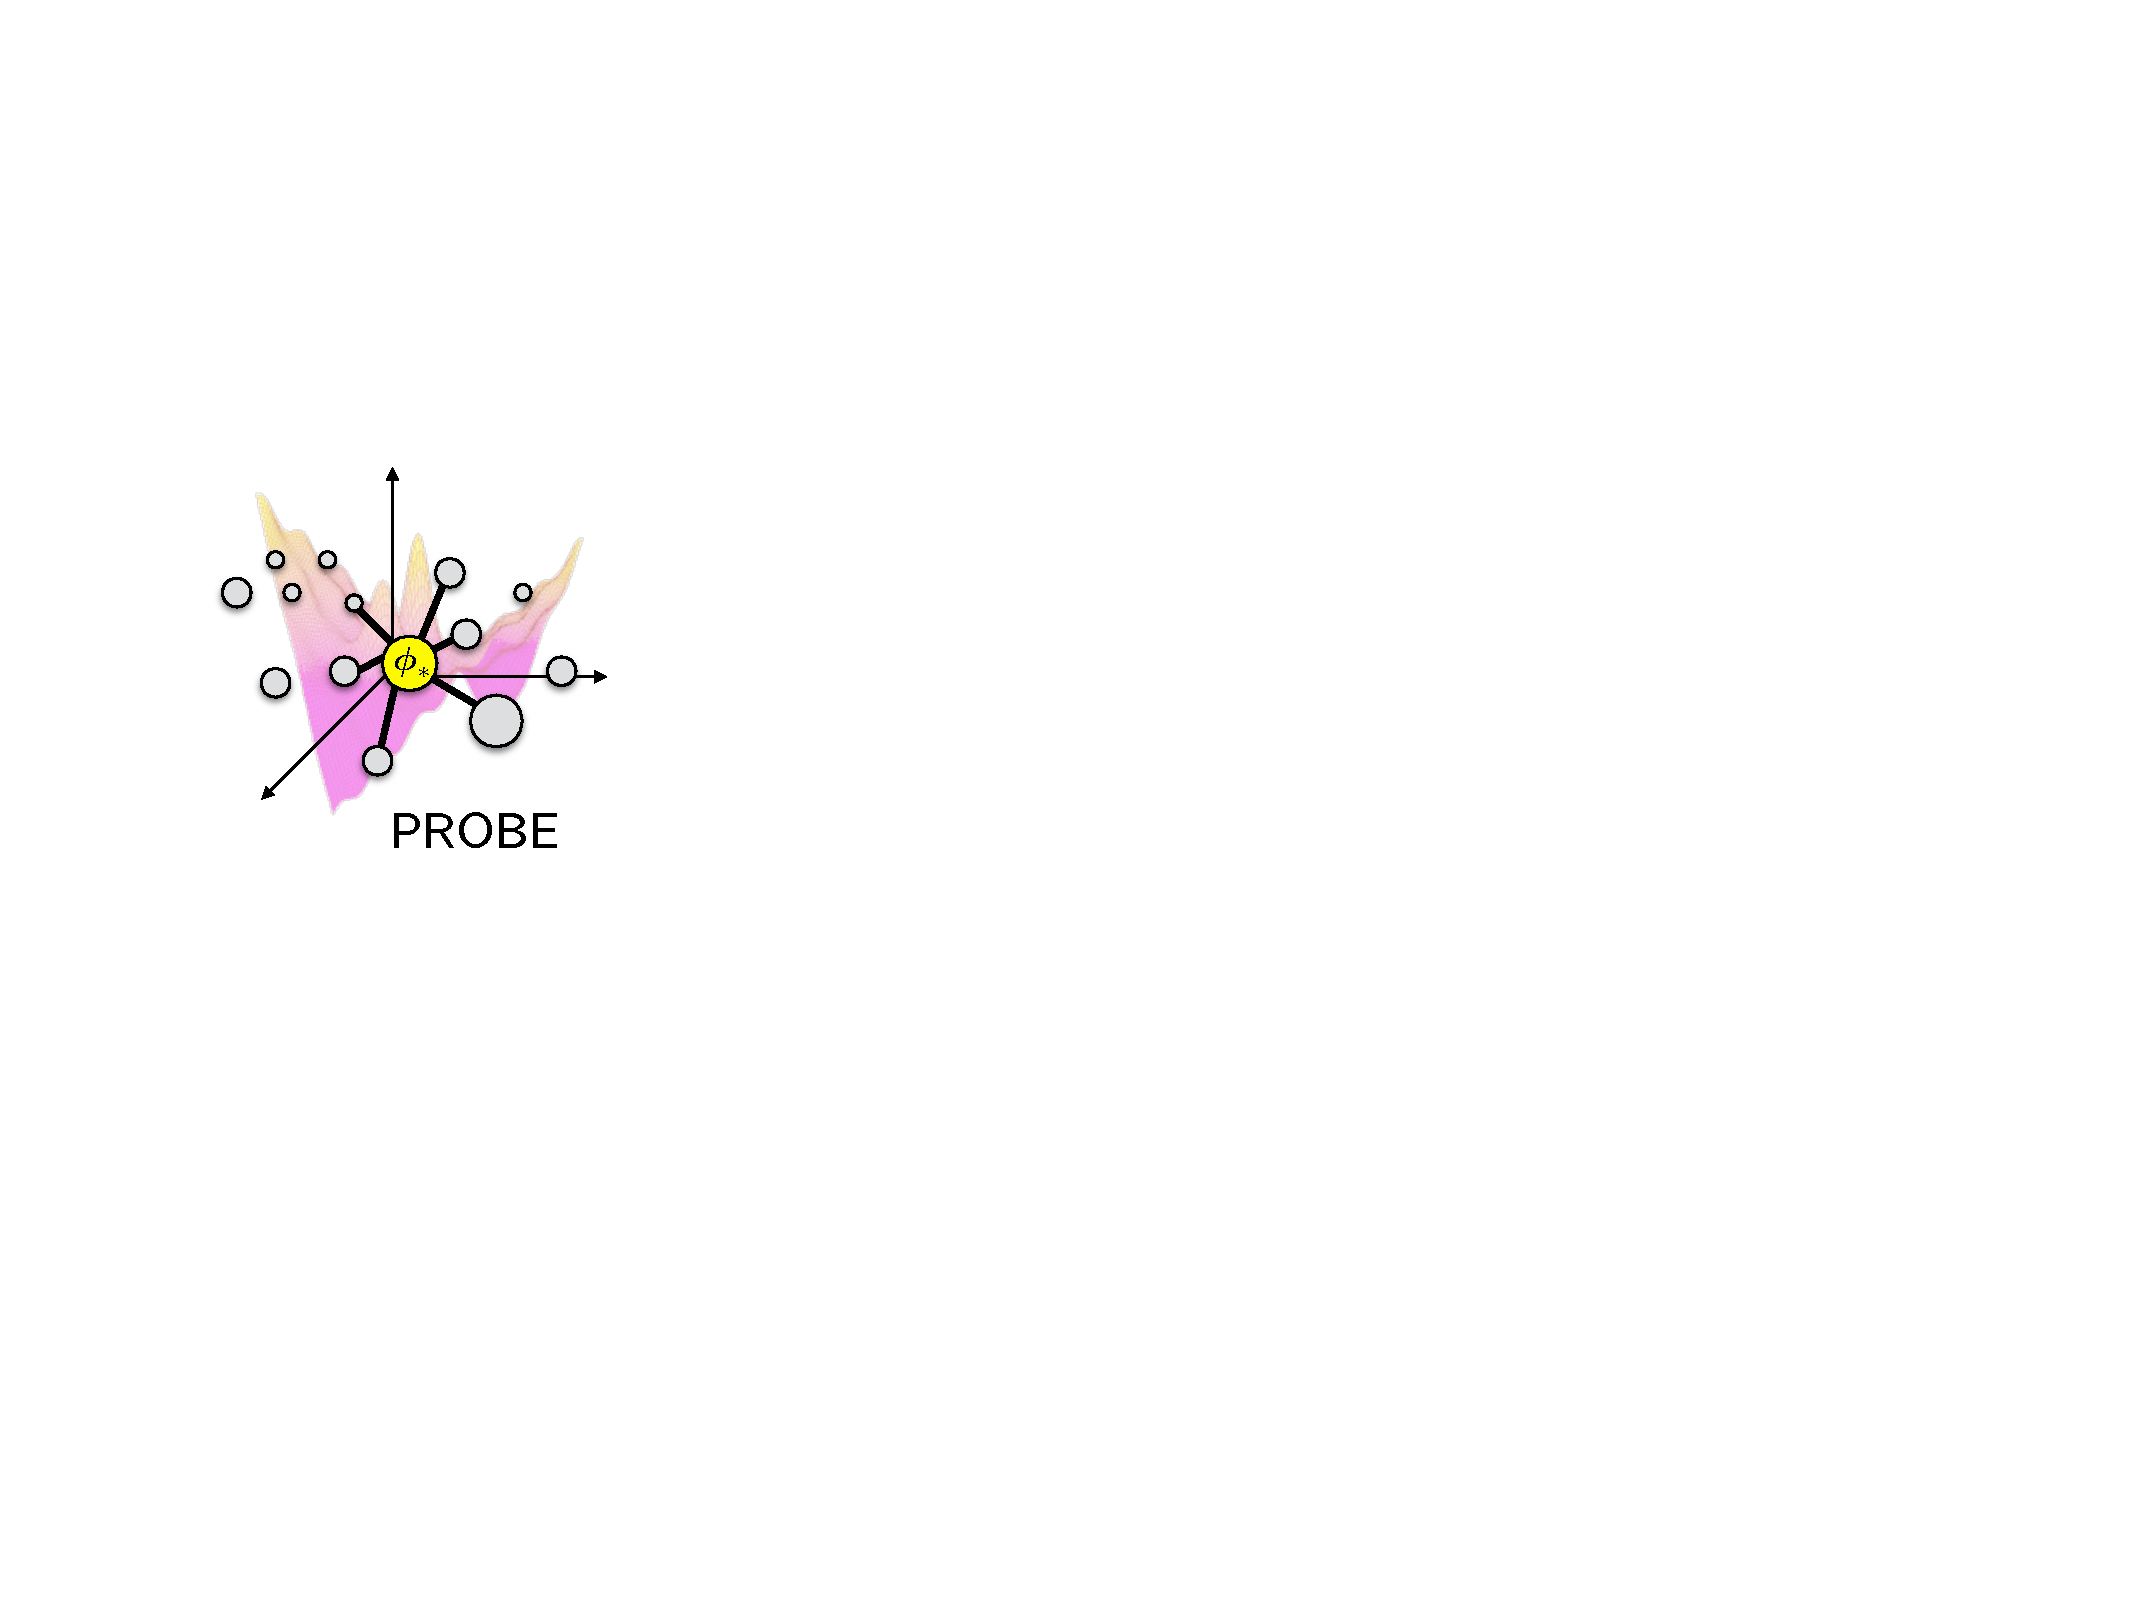
\includegraphics[width=0.8\textwidth]{probe.pdf}
 \caption{PROBE builds a predictive noise model for stereo visual odometry.}
 \label{fig:probe_intro_fig}
\end{figure*}

The first pseudo-sensor we present is a general technique we call PRedictive ROBust Estimation, or PROBE. This approach uses non-parametric learning to predict observation covariances for a stereo visual odometry pipeline, effectively scaling a least squares objective in a predictive fashion. We present two different methods to learn and incorporate these covariances. First we use a simple k-nearest-neighbours approach to learn isotropic covariances for three dimensional point-cloud matching. Second, we extend this significantly by applying the method of Generalized Kernels to a Bayesian treatment of covariance learning. We show that by assuming a particular covariance prior over re-projection errors, we can derive a robust least squares loss with parameters that are predicted for each  error by our approach.

There are three publications associated with this work:
\begin{enumerate}
\item \bibentry{2015_Peretroukhin_PROBE}
\item \bibentry{2015_Peretroukhin_Get}
\item \bibentry{Peretroukhin2016-om}.
\end{enumerate}



%\begin{wrapfigure}{r}{0.5\textwidth}
%    \centering
%      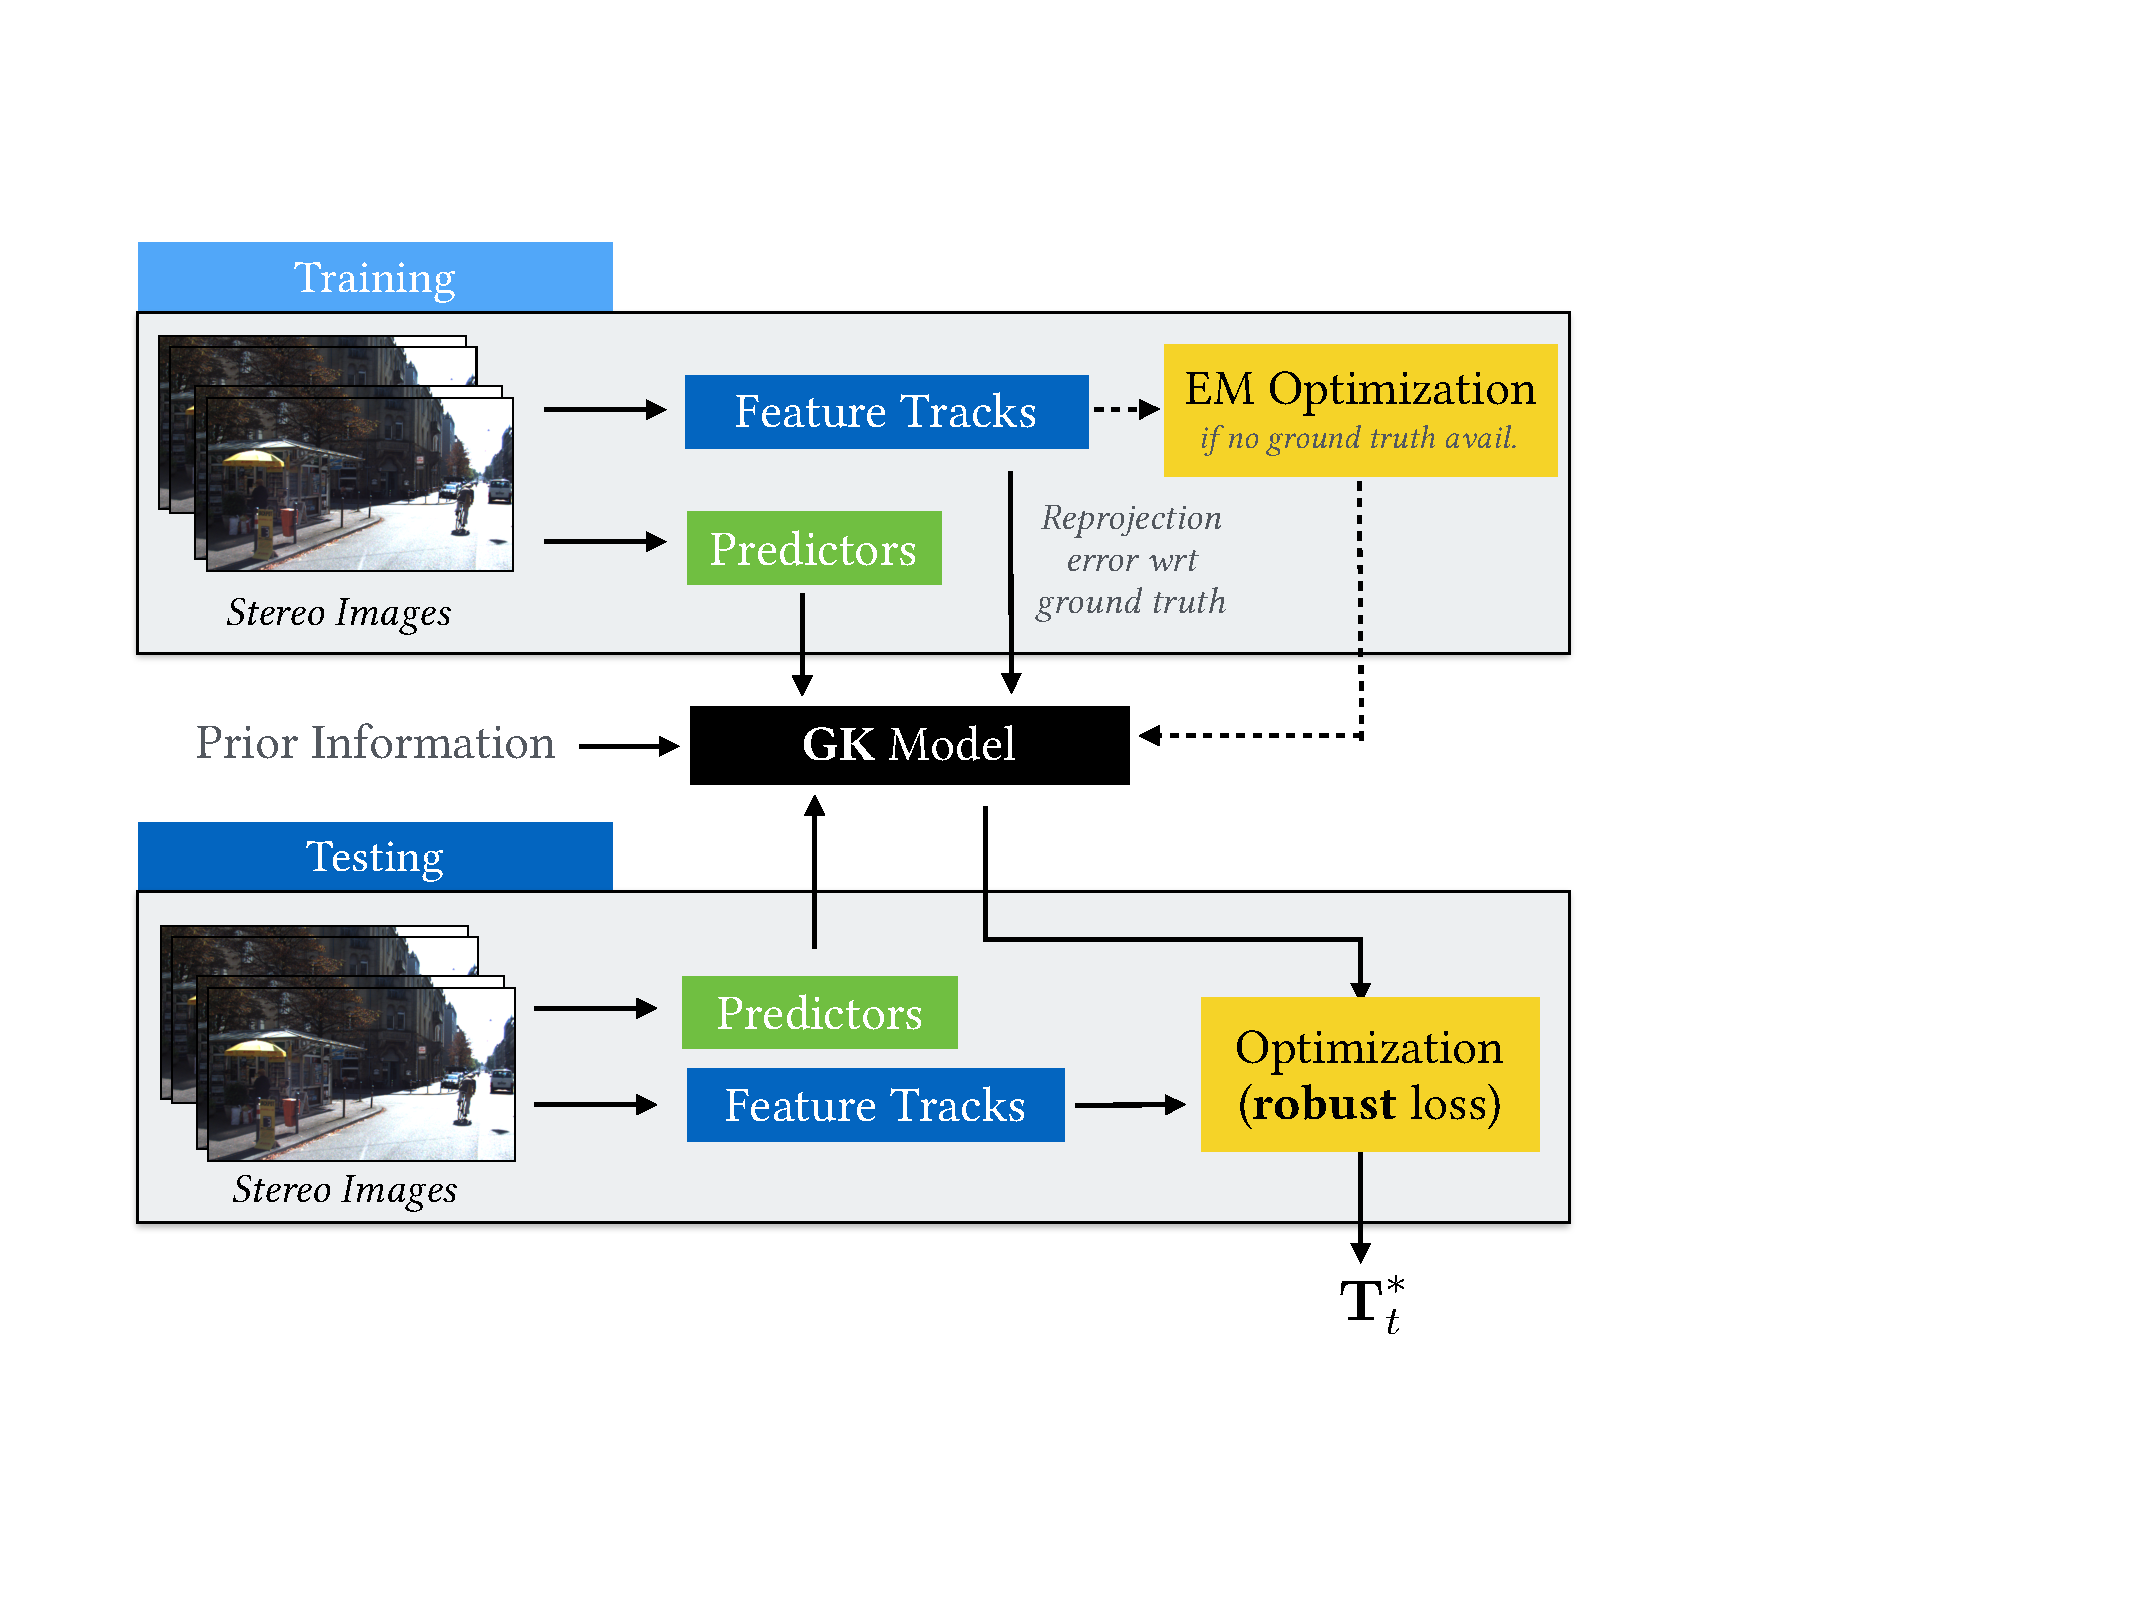
\includegraphics[width=0.5\textwidth]{probe-gk/system_overview}
%      \caption{PROBE builds a predictive noise model for stereo visual odometry.}
%        \vspace{-1em}
%    \label{fig:probe_gk_system}
%\end{wrapfigure}

\section{Motivation}

Robot navigation relies on an accurate quantification of sensor noise or uncertainty in order to produce reliable state estimates.
In practice, this uncertainty is often fixed for a given sensor and experiment, whether by automatic calibration or by manual tuning.
Although a fixed measure of uncertainty may be reasonable in certain static environments, dynamic scenes frequently exhibit many effects that corrupt a portion of the available observations.
For visual sensors, these effects include, for example, self-similar textures, variations in lighting, moving objects, and motion blur. 
We assert that there may be useful information available in these observations that would normally be rejected by a fixed-threshold outlier rejection scheme. 
Ideally, we would like to retain some of these observations in our estimator, while still placing more trust in observations that do not suffer from such effects.

\section{Related Work}


There is a large and growing body of work on the problem of deriving accurate,
consistent state estimates from visual data.  Although our approach to noise
modelling is applicable in other domains, for simplicity we focus our attention
on the problem of inferring egomotion from features extracted from sequential
pairs of stereo images; see \citet{sunderhauf2007stereo} for a survey of
techniques. The spectrum of alternative approaches to visual state estimation
include monocular techniques, which may be feature-based
\citep{scaramuzza2011visual}, direct \citep{irani2000direct}, or semi-direct
\citep{forster2014svo}. 

Apart from simply rejecting outliers, a number of recent approaches attempt to
select the optimal set of features to produce an accurate localization estimate
from tracked visual features. For example, \citet{Tsotsos2015} amend Random
Sample Consensus (RANSAC) with statistical hypothesis testing to ensure that tracked visual features have normally distributed residuals before including them in
the estimator. Unlike our predictive approach, their technique relies on the availability of feature tracks, and requires scene overlap to work continuously. In a different
approach, \Citet{Zhang2015} choose an optimally observable feature subset for a
monocular SLAM pipeline by selecting features with the highest \textit{informativeness} - a measure calculated based on the observability of the SLAM subsystem. Observability, however, is governed by the 3D location of the features, and therefore cannot predict systematic feature degradation due to environmental or sensor-based effects. 

\section{PROBE: Scalar k-Nearest Neighbours}

In our initial exploratory work, we explored the idea of scaling 
With Predictive ROBust Estimation, we aim to improve localization accuracy in the presence of such effects by building a model of the uncertainty in the affected visual observations. 
We learn the model in an offline training procedure and then use it online to predict the uncertainty of incoming observations as a function of their location in a predefined \emph{prediction space}.
Our model can be learned in completely unknown environments with frequent or infrequent ground truth data.
 

The primary contributions of this research are a flexible framework for learning the quality of visual features with respect to navigation estimates, and a straightforward way to incorporate this information into a navigation pipeline. On its own, PROBE can produce more accurate estimates than a binary outlier rejection scheme like Random Sample Consensus (RANSAC) because it can simultaneously reduce the influence of outliers while intelligently weighting inliers. PROBE reduces the need to develop finely-tuned uncertainty models for complex sensors such as cameras, and better accounts for the effects observed in complex, dynamic scenes than typical fixed-uncertainty models. While we present PROBE in the context of visual feature-based navigation, we stress that it is not limited to visual measurements and could also be applied to other sensor modalities.
% The remainder of this paper is organized as follows: In Section \ref{sec:related_work}, we discuss related work in the literature. Section \ref{sec:approach} outlines our tightly-coupled visual-inertial odometry pipeline and learning model. Section \ref{sec:predictors} discusses and justifies our choice of prediction space. Sections \ref{sec:results} and \ref{sec:discussion} discuss experimental results of PROBE's performance on several segments from the KITTI dataset \cite{Geiger:2013kp}, and experimental datasets collected at the University of Toronto Institute for Aerospace Studies (UTIAS). Finally, Section \ref{sec:conclusions} offers some concluding remarks.



The aim of PROBE is to learn a model for the quality of visual features, with the goal of reducing the impact of deleterious visual effects such as moving objects, motion blur, and shadows on navigation estimates.
Feature quality is characterized by a scalar weight, $\beta_i$, for each visual feature in an environment.
To compute $\beta_i$ we define a prediction space (similar to \cite{VegaBrown:ew}) that consists of a set of visual-inertial predictors computed from the local image region around the feature and the inertial state of the vehicle (Section \ref{sec:predictors} details our choice of predictors).
We then scale the image covariance of each feature by $\beta_i$ during the non-linear optimization.

In a similar manner to M-estimation, PROBE achieves robustness by varying the influence of certain measurements.
However, in contrast to robust cost functions that weight measurements based purely on estimation error, PROBE weights measurements based on their assessed quality.

To learn the model, we require training data that consists of a traversal through a typical environment with some measure of ground truth for the path, but not for the visual features themselves. Like many machine learning techniques, we assume that the training data is representative of the test environments in which the learned model will be used. 

We learn the quality of visual features \textit{indirectly} through their effect on navigation estimates. We define high quality features as those that result in estimates that are close to ground truth. Our framework is flexible enough that we do not require ground truth at every image and we can learn the model based on even a single loop closure error.


\subsection{Mathematical Formulation}



To solve for the relative egomotion between two camera frames, $\CoordinateFrame{c_0}$ and $\CoordinateFrame{c_1}$, we follow technique described in \Cref{sec:vo_point_cloud} to convert stereo observations into point-clouds and then solve for the maximum likelihood $\LieGroupSE{3}$ transformation. We associate with each match $\{\ImageLandmark{i}{c_0}, \ImageLandmark{i}{c_1}\}$ a vector of
\emph{predictors}, $\Predictor{i}{c}$.  Each predictor can be computed using both visual\footnote{Including potentially data from all four images in the pair of stereo images.} and inertial cues , allowing us to model effects like motion blur and self-similar
textures. We then compute the covariance as a function of these predictors, so
that $\ImageLandmarkCovariance{i}{c} = \Covariance( \Predictor{i}{c})$, and we use the same covariance function for features in both frames\footnote{We conjecture that this is reasonable in a VO setup, where images change minimally between consecutive frames.},
\begin{align}
	\ImageLandmark{i}{c_0} &\sim \NormalDistribution\left(\bar{\Vector{y}}_{i,c_0}, \ImageLandmarkCovariance{i}{c} \right) = \NormalDistribution\left(\bar{\Vector{y}}_{i,c_0}, \Covariance( \Predictor{i}{c})\right) \\
		\ImageLandmark{i}{c_1} &\sim \NormalDistribution\left(\bar{\Vector{y}}_{i,c_1}, \ImageLandmarkCovariance{i}{c} \right) = \NormalDistribution\left(\bar{\Vector{y}}_{i,c_1}, \Covariance( \Predictor{i}{c})\right)
\end{align}


This then builds the following weighted least squares objective,

\begin{equation}
\label{eq:vo_objective}
  \Transform_t^* = \ArgMin{\Transform\in\text{SE}(3)}\sum_{i=1}^{N_t} 
  \Transpose{\Vector{e}_{i}(\Transform_t)} \GeneralCovariance_{i,t}^{-1} \Vector{e}_{i}(\Transform_t).
\end{equation}
where $\GeneralCovariance_{i,t}$ is now given by,
\begin{equation}
	\GeneralCovariance_{i,t} = \Matrix{D}\Matrix{G}_{i,c_1} \Covariance( \Predictor{i}{c})  \Matrix{G}_{i,c_1}^T \Matrix{D}^T + 
 \Matrix{D}\Transform_t \Matrix{G}_{i,c_0} \Covariance( \Predictor{i}{c}) \Matrix{G}_{i,c_0}^T  \Transform_t^T \Matrix{D}^T
\end{equation}
We build a model for $\Covariance( \Predictor{i}{c})$ as,
\begin{equation}
\Covariance( \Predictor{i}{c}) = \beta(\Predictor{i}{c}) \bar{\Covariance},
\end{equation}
with
\begin{equation}
 \beta(\Predictor{i}{c}) = \left(\frac{1}{\PROBEPoseError_\text{avg} K} \sum_{k=1}^K \PROBEPoseError_k  \right)^{\gamma}, ~ \PROBEPoseError_k \in \textsc{k-NN}(\Predictor{i}{c}),
\end{equation}

where $\{\PROBEPoseError_k\}_{k=1}^K$ are $K$ egomotion errors that are `nearest' to $\Predictor{i}{c}$, $\epsilon_\text{avg}$ is an average error, and $\gamma > 1$ is a hyper-parameter designed to exaggerate the effect of small changes in position error.

\subsection{Training}
Training proceeds by traversing the training path, selecting a subset of visual features at each step, and using them to compute an incremental position estimate. By comparing the estimated position to the ground truth position, we compute the translational Root Mean Squared Error (RMSE), $\epsilon$, and store it at each feature's position in the prediction space. The full algorithm is summarized in \Cref{alg:probe_train}. 
%\begin{figure}[h]
%\begin{center}
%\begin{algorithmic}[1]
%\Procedure{trainPROBE}{}
%\For{$l\gets 1, N_{iter}$}
%\For{$s\gets 1, N_{path}$}
%	\State $f_1, \dots, f_J \gets \text{samplefeatures}(l)$
%	\State $\mbs\pi^1_l, \dots, \mbs\pi^J_l \gets predictors(f_1, \dots, f_J)$
%	\State $\bar{\mbf{C}}_{ba},  \bar{\mbf{r}}_a^{ba} \gets poseChange(f_1, \dots, f_J)$
%	\State $\mbf \alpha_{l,s}  \gets computeRMSE(\bar{\mbf{r}}_a^{ba}, {\mbf{r}_{a}^{ba}}_{GT} )$
%	\State  $ \Theta_{l,s} \gets \left\{\mbs\pi^1_{l,s}, \dots, \mbs\pi^J_{l,s}, \alpha_{l,s}\right\}$
%\EndFor
%\EndFor
%\State \textbf{return} $\mbs \Theta = \{ \Theta_{l,s} \}$
%\EndProcedure
%\end{algorithmic}
%\caption{The PROBE training procedure.}\label{fig:ProbeTraining}
%\end{center}
%\end{figure}

\begin{algorithm}
  \caption{Train PROBE based on a dataset ($\mathcal{D}$) of pairs of input sensor data ($\mathcal{I}_s$) and ground truth egomotion ($\Transform_s$).}
   \label{alg:probe_train}
  \begin{algorithmic}
    \Function{BuildPROBEModel}{$\mathcal{D}$}
      \For{$l \gets [1,...,N_{iter}]$}
      \ForAll{$\mathcal{I}_s$, $\Transform_s$ in $\mathcal{D}$}
	\State $\mathcal{F} \gets$ \Call{extractFeatures}{$\mathcal{I}_s$}
	\State $\{f_1, \dots, f_J\} \gets$ \Call{sample}{$\mathcal{F}$}
	\State $\Estimate{\Transform} \gets$ \Call{computeTransform}{$\{f_1, \dots, f_J\}$}
	\State $\mbf \PROBEPoseError  \gets$ \Call{error}{$\Estimate{\Transform}, \Transform_s$}
	\State $\{\Predictor{s}{1}, \dots, \Predictor{s}{J}\} \gets$ \Call{predictor}{$\{f_1, \dots, f_J\}$}
	\State Insert $\{\Predictor{s}{1}, \dots,  \Predictor{s}{J}\}$ into $\mathcal{M}$ and store $\PROBEPoseError$ at all $J$ locations
	\EndFor
      \EndFor
      \State\Return  $\mathcal{M}$
    \EndFunction
  \end{algorithmic}
\end{algorithm}

	\subsection{Evaluation}
To use the PROBE model in a test environment, we compute the location of each observed visual feature in our prediction space, and then compute its relative weight $\beta_i$ as a function of its $K$ nearest neighbours in the training set.
For efficiency, the $K$ nearest neighbours are found using a $k$-d tree.
The final scaling factor $\beta_i$ is a function of the mean of the $\alpha$ values corresponding to the $K$ nearest neighbours, normalized by $\PROBEPoseError_\text{avg}$, the mean $\alpha$ value of the entire training set.

\begin{algorithm}
  \caption{Compute scalar covariance factors, $\beta_i$, for a set of stereo feature tracks (and IMU data), $\mathcal{F}$, given a PROBE model $\mathcal{M}$.}
  \label{alg:probe_test}
  \begin{algorithmic}
    \Function{UsePROBE}{$\mathcal{M}$, $\mathcal{F}, \gamma$}
     \State $\PROBEPoseError_\text{avg} \gets$ \Call{averageError}{$\mathcal{M}$}
      \ForAll{$f_i$ in $\mathcal{F}$}
        \State $\Vector{\phi}_i \gets$ \Call{predictor}{$f_i$} 
        \State $\PROBEPoseError_1,...,\PROBEPoseError_K \gets$ \Call{findKNN}{$\Vector{\phi}_i, K, \mathcal{M}$}
		\State $\beta_i \gets \left(\frac{1}{\PROBEPoseError_\text{avg} K} \sum_{k=1}^K \PROBEPoseError_k  \right)^{\gamma}$
		
	   \EndFor
      \State\Return $\mbs \beta = \{\beta_i\}$
    \EndFunction
  \end{algorithmic}
\end{algorithm}


The value of $K$ can be determined through cross-validation, and in practice depends on the size of the training set and the environment.
The computation of $\beta_i$ is designed to map small differences in learned $\alpha$ values to scalar weights that span several orders of magnitude.
An appropriate value of $\gamma$ can be found by searching through a set range of candidate values and choosing the value that minimizes the average RMSE (ARMSE) on the training set.


\subsection{Prediction Space} \label{sec:predictors}
A crucial component of our technique is the choice of prediction space.
In practice, feature tracking quality is often degraded by a variety of effects such as motion blur, moving objects, and textureless or self-similar image regions.
% Features suffering from such effects are often poorly localized in the image, yet may contain useful information that we would like to retain in our estimator.
% Conversely, we would like to place more trust in features that do not suffer from such effects.
The challenge is in determining predictors that account for such effects without requiring excessive computation.
In our implementation, we use the following predictors, but stress that the choice of predictors can be tailored to suit particular applications and environments:
\begin{itemize}
    \item Angular velocity and linear acceleration magnitudes
    \item Local image entropy
    \item Blur (quantified by the blur metric of \cite{crete2007blur})
    \item Optical flow variance score
    \item Image frequency composition
\end{itemize}
We discuss each of these predictors in turn.


\subsubsection{Angular velocity and linear acceleration}
While most of the predictors in our system are computed directly from image data, the magnitudes of the angular velocities and linear accelerations reported by the IMU are in themselves good predictors of image degradation (e.g., image blur) and hence poor feature tracking. 
%We do not explicitly correct for bias in linear accelerations because we expect real motion-induced acceleration to trump bias at the timescales of our test trials.  As a result, there is virtually no computational cost involved in incorporating these quantities as predictors.

\subsubsection{Local image entropy}
Entropy is a statistical measure of randomness that can be used to characterize the texture in an image or patch.
Since the quality of feature detection is strongly influenced by the strength of the texture in the vicinity of the feature point, we expect the entropy of a patch centered on the feature to be a good predictor of its quality.
We evaluate the entropy $S$ in an image patch by sorting pixel intensities into $N$ bins and computing
\begin{equation}
    S = -\sum_{i=1}^N c_i \log_2(c_i),
\end{equation}
where $c_i$ is the number of pixels counted in the $i^\text{th}$ bin.


\subsubsection{Blur}
Blur can arise from a number of sources including motion, dirty lenses, and sensor defects.
All of these have deleterious effects on feature tracking quality.
To assess the effect of blur in detail, we performed a separate experiment.
We recorded images of 32 interior corners of a standard checkerboard calibration target using a low frame-rate (20 FPS) Skybotix VI-Sensor stereo camera and a high frame-rate (125 FPS) Point Grey Flea3 monocular camera rigidly connected by a bar (\Cref{fig:probe_tricifix}).
Prior to the experiment, we determined the intrinsic and extrinsic calibration parameters of our rig using the \textsc{Kalibr}\footnote{\url{https://github.com/ethz-asl/kalibr}} package \cite{Furgale2013-sl}.
The apparatus underwent both slow and fast translational and rotational motion, which induced different levels of motion blur as quantified by the blur metric proposed by \cite{crete2007blur}.
% The two motion regimes induced different levels of motion blur, which we distinguish by thresholding the blur metric proposed by \cite{Anonymous:Ngi3VEEU}.

\begin{figure}
    \centering
    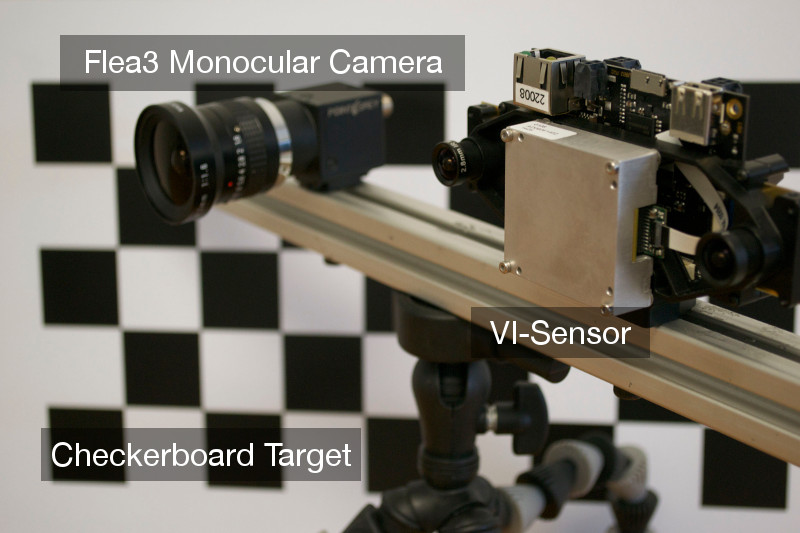
\includegraphics[width=0.4\textwidth]{probe/tricifix2}
    \caption{The Skybotix VI-Sensor, Point Grey Flea3, and checkerboard target used in our motion blur experiments.}
    \label{fig:probe_tricifix}
\end{figure}

%\begin{figure}
%    \centering
%    \includegraphics[width=0.4\textwidth]{figs/blurMetric_short}
%    \caption{Blur metric \cite{Anonymous:Ngi3VEEU} computed for the left camera of the VI-Sensor for the checkerboard dataset. We separate the dataset into regions of high and low blur corresponding to fast and slow motion, respectively.}
%    \label{fig:visensor_blurMetric}
%\end{figure}


\begin{figure}
    \centering
        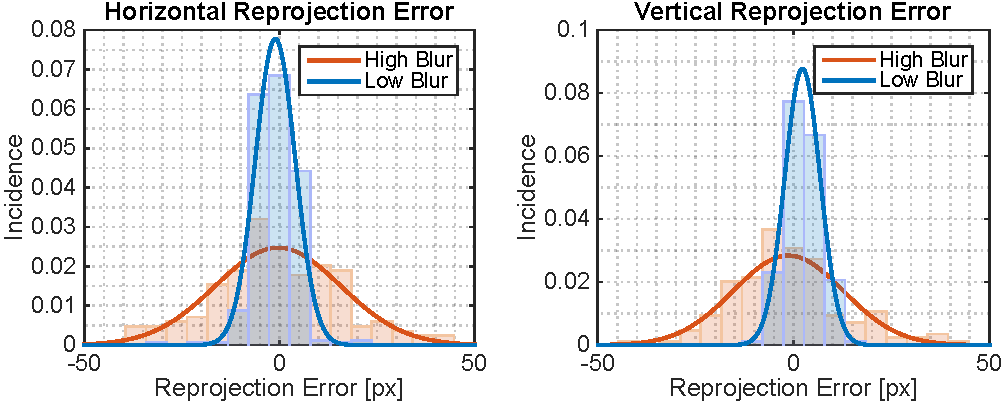
\includegraphics[width=0.85\textwidth]{probe/reprojectionError}
        \label{fig:probe_visensor_reprojectionError}
      \caption{Reprojection error of checkerboard corners triangulated from the VI-Sensor and reprojected into the Flea3.}
\end{figure}

\begin{figure}
    \centering
    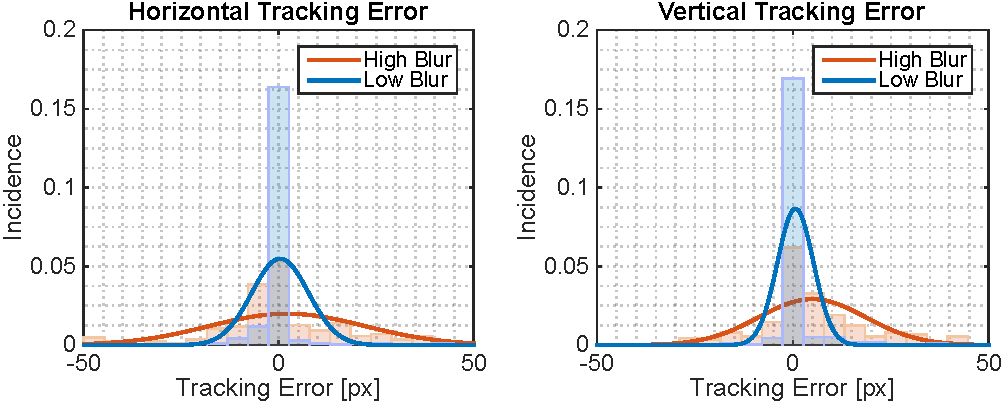
\includegraphics[width=0.85\textwidth]{probe/trackingError}
    \label{fig:probe_visensor_trackingError}
    \caption{Effect of blur on reprojection and tracking error for the slow-then-fast checkerboard dataset. We distinguish between high and low blur by thresholding the blur metric \cite{crete2007blur}. The variance in both errors increases with blur.}
    \label{fig:probe_visensor_histograms}
\end{figure}

We detected checkerboard corners in each camera at synchronized time steps, computed their 3D coordinates in the VI-Sensor frame, then reprojected these 3D coordinates into the Flea3 frame.
We then computed the reprojection error as the distance between the reprojected image coordinates and the true image coordinates in the Flea3 frame.
Since the Flea3 operated at a much higher frame rate than the VI-Sensor, it was less susceptible to motion blur and so we treated its observations as ground truth.
We also computed a tracking error by comparing the image coordinates of checkerboard corners in the left camera of the VI-Sensor computed from both KLT tracking \cite{Lucas:1981} and re-detection.

\Cref{fig:probe_visensor_histograms} shows histograms and fitted normal distributions for both reprojection error and tracking error.
From these distributions we can see that the errors remain approximately zero-mean, but that their variance increases with blur.
This result is compelling evidence that the effect of blur on feature tracking quality can be accounted for by scaling the feature covariance matrix by a function of the blur metric.


\subsubsection{Optical flow variance score}
To detect moving objects, we compute a score for each feature based on the ratio of the variance in optical flow vectors in a small region around the feature to the variance in flow vectors of a larger region.
Intuitively, if the flow variance in the small region differs significantly from that in the larger region, we might expect the feature in question to belong to a moving object, and we would therefore like to trust the feature less.
Since we consider only the variance in optical flow vectors, we expect this predictor to be reasonably invariant to scene geometry.

We compute this optical flow variance score according to
\begin{equation}
    \log \left( \frac{\bar{\sigma}^2_s}{\bar{\sigma}^2_l} \right),
\end{equation}
where $\bar{\sigma}^2_s, \bar{\sigma}^2_l$ are the means of the variance of the vertical and horizontal optical flow vector components in the small and large regions respectively.
\Cref{fig:probe_flow_variance} shows sample results of this scoring procedure for two images in the KITTI dataset.
Our optical flow variance score generally picks out moving objects such as vehicles and cyclists in diverse scenes.

\begin{figure}
    \centering
    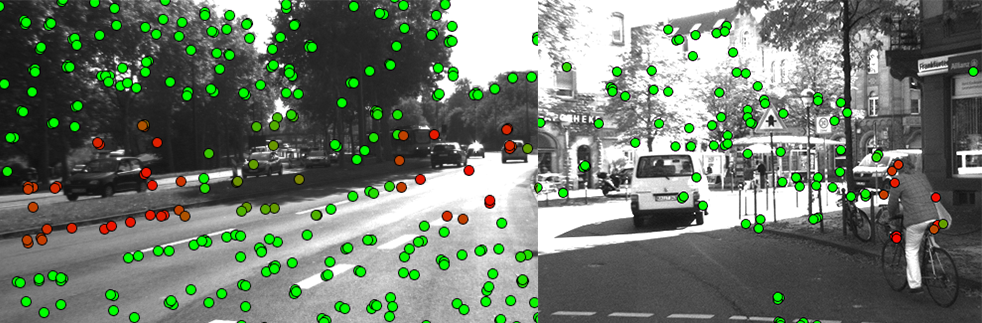
\includegraphics[width=0.8\textwidth]{probe/flowPredictorCombined.png}
    \caption{The optical flow variance predictor can help in detecting moving objects. Red circles correspond to higher values of the optical flow variance score (i.e., features more likely to belong to a moving object).}
    \label{fig:probe_flow_variance}
\end{figure}

\subsubsection{Image frequency composition}
Reliable feature tracking is often difficult in textureless or self-similar environments due to low feature counts and false matches.
We detect textureless and self-similar image regions by computing the Fast Fourier Transform (FFT) of each image and analyzing its frequency composition.
For each feature, we compute a coefficient for the low- and high-frequency regimes of the FFT.
\Cref{fig:probe_high_frequency} shows the result of the high-frequency version of this predictor on a sample image from the KITTI dataset.
Our high-frequency predictor effectively distinguishes between textureless regions (e.g., shadows and roads) and texture-rich regions (e.g., foliage).


\begin{figure}
    \centering
    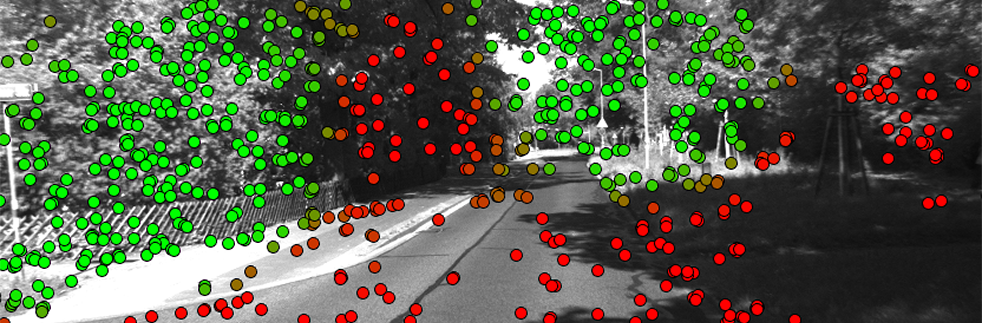
\includegraphics[width=0.8\textwidth]{probe/highFreqPredictor.png}
    \caption{A high-frequency predictor can distinguish between regions of high and low texture such as foliage and shadows. Green indicates higher values.}
    \label{fig:probe_high_frequency}
\end{figure}



\begin{table}
    \centering
    
    \caption{Comparison of translational Average Root Mean Square Error (ARMSE) and Final Translational Error on the KITTI dataset.}
	\resizebox{\columnwidth}{!}{%
    % Need to add an asterisk to the 30_drive_0027 "Type" to indicate that it's trained on City data, but can't do it without messing up the justification - Matt
    \begin{threeparttable}
        \begin{tabular}{cccccccccccc}
        & & & & \multicolumn{2}{c}{Nominal RANSAC} & & \multicolumn{2}{c}{Aggressive RANSAC} & & &  \\
        	 & & & & \multicolumn{2}{c}{(99\% outlier rejection)} & & \multicolumn{2}{c}{(99.99\% outlier rejection)} & & \multicolumn{2}{c}{PROBE} \B \\
             \cline{5-6} \cline{8-9} \cline{11-12}
        	 Trial & Type & Path Length &&  ARMSE & Final Error & & ARMSE & Final Error & & ARMSE & Final Error \T\B \\ \hline \T
        	\texttt{26\_drive\_0051} & City \tnote{1} & 251.1 m && 4.84 m & 12.6 m && 3.30 m & 8.62 m && 3.48 m & 8.07 m \\
        	\texttt{26\_drive\_0104} & City \tnote{1} & 245.1 m && 0.977 m & 4.43 m && 0.850 m & 3.46 m && 1.19 m & 3.61 m \\ 
        	\texttt{29\_drive\_0071} & City \tnote{1} & 234.0 m && 5.44 m & 30.3 m && 5.44 m & 30.4 m && 3.03 m & 12.8 m \\ 
        		\texttt{26\_drive\_0117} & City \tnote{1} & 322.5 m && 2.29 m & 9.07 m && 2.29 m & 9.07 m && 2.76 m & 9.08 m \\ 
        		\texttt{30\_drive\_0027} & Residential \tnote{1, \dag} & 667.8 m && 4.22 m & 12.2 m && 4.30 m & 10.6 m && 3.64 m & 4.57 m \\ 
        		\texttt{26\_drive\_0022} & Residential \tnote{2} & 515.3 m && 2.21 m & 3.99 m && 2.66 m & 6.09 m && 3.06 m & 4.99 m \\ 
        		\texttt{26\_drive\_0023} & Residential \tnote{2} & 410.8 m && 1.64 m & 8.20 m && 1.77 m & 8.27 m && 1.71 m & 8.13 m \\ 
        		\texttt{26\_drive\_0027} & Road \tnote{3} & 339.9 m && 1.63 m & 8.75 m && 1.63 m & 8.65 m && 1.40 m & 7.57 m \\ 
        		\texttt{26\_drive\_0028} & Road \tnote{3} & 777.5 m && 4.31 m & 16.9 m && 3.72 m & 13.1 m && 3.92 m & 13.2 m \\ 
        		\texttt{30\_drive\_0016} & Road \tnote{3} & 405.0 m && 4.56 m & 19.5 m && 3.33 m & 14.6 m && 2.76 m & 13.9 m \\ 
                UTIAS Outdoor & Snowy parking lot & 302.0 m && 7.24 m & 10.1 m && 7.02 m & 10.6 m && 6.85 m & 6.09 m \\ 
                UTIAS Indoor & Lab interior & 32.83 m && --- & 0.854 m && --- & 0.738 m && --- & 0.617 m  \B \\    
        \hline
            \label{table:probe_kitti_data}
        \end{tabular}
        \begin{tablenotes}
            \item[1] Trained using sequence \texttt{09\_26\_drive\_0005}. ~$^2$ Trained using sequence  \texttt{09\_26\_drive\_0046}. ~$^3$ Trained using sequence  \texttt{09\_26\_drive\_0015}.  
            \item[\dag] This residential trial was evaluated with a model trained on a sequence from the city category because of several moving vehicles that were better represented in that training dataset.
        \end{tablenotes}
    \end{threeparttable}
    }
\end{table}

\begin{figure}
    \centering
    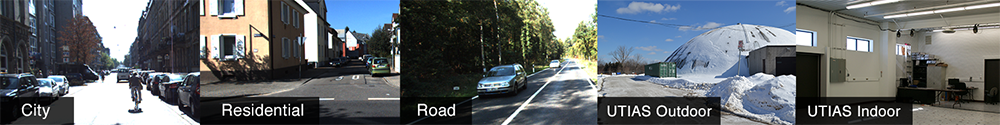
\includegraphics[width=\textwidth]{probe/city-res-road.png}
    \caption{Three types of environments in the KITTI dataset, as well as 2 types of environments at the University of Toronto.  We use one trial from each category to train and then evaluate separate trials in the same category.}
    \label{fig:probe_KITTI-Types}
\end{figure}

\begin{figure}
    \centering
    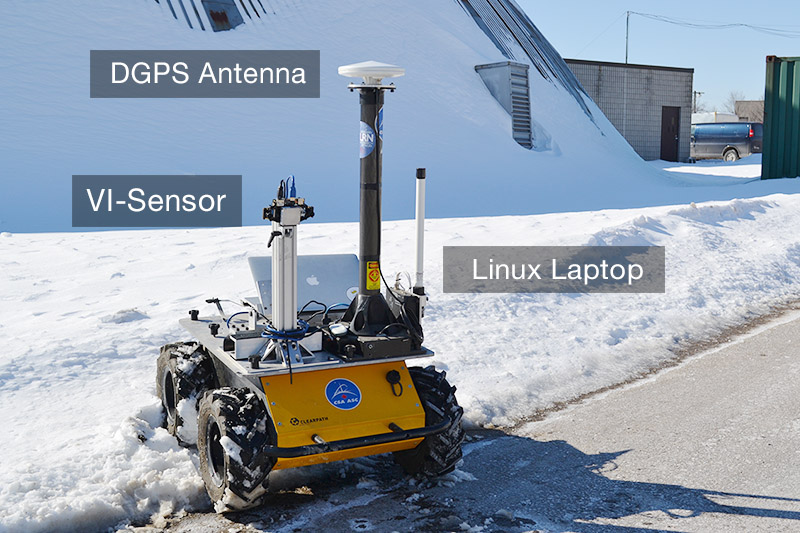
\includegraphics[width=0.6\textwidth]{probe/husky2}
    \caption{Our four-wheeled skid-steered Clearpath Husky rover equipped with Skybotix VI-Sensor and Ashtech DGPS antenna used to collect the outdoor UTIAS dataset.}
    \label{fig:probe_huskypic}
\end{figure}

\section{Generalized Kernels}

However, not all features are created equal; most feature-based methods rely on
random sample consensus algorithms \citep{fischler1981random} to partition the extracted features
into inliers and outliers, and perform estimation based only on inliers. It is
common to guard against misclassifying an outlier as an inlier by using robust
estimation techniques, such as the Cauchy costs employed in
\citet{kerl2013robust} or the dynamic covariance scaling devised
by \citet{Burgard:ii}. These approaches, often grouped under the title of M-estimation, aim to maintain a quadratic influence
of small errors, while reducing the contribution of larger errors. The
robustness and accuracy of feature-based visual odometry often hinges on the
tuning of the parameters of inlier selection and robust estimation. Performance
can vary significantly from one environment to the next, and most algorithms require
careful tuning to work in a given environment. 

In this work, we describe a principled, data-driven way to build a noise model
for visual odometry. We combine our previous work \citep{peretroukhin2015PROBE}
on predictive robust estimation (PROBE) with our work on covariance estimation
\citep{VegaBrown:2013fv} to formulate a predictive robust estimator for a
stereo visual odometry pipeline. We frame the traditional non-linear least
squares optimization problem as a problem of maximum likelihood estimation with
a Gaussian noise model, and infer a distribution over the covariance matrix of
the Gaussian noise from a predictive model learned from training data. This
results in a Student's~$t$ distribution over the noise, and naturally yields a
robust nonlinear least-squares optimization problem.  In this way, we can predict,
in a principled manner, how informative each visual feature is with respect to the final state
estimate, which allows our approach to intelligently weight observations to
produce more accurate odometry estimates.  Our pipeline is outlined in
Figure \ref{fig:probe_gk_system}.

\subsection{Predictive noise models for visual odometry}
%
%The process described in the previous section employs a fixed noise covariance
%$\Covariance$.  However, not all landmarks are created equal: differing texture
%gradients can cause feature localization to degrade in predictable ways, and
%effects like motion blur can lead to landmarks being less informative. If we had a
%good estimate of the noise covariance for each landmark, we could simply replace the fixed covariance $\Covariance$
%with one that varies for each stereo observation,
%$\ImageLandmarkCovariance{i}{t}$. Such a predictive model would allows us to  better account for observation errors from a diverse set of noise sources, and incorporate information from landmarks that may otherwise be discarded by a binary outlier rejection scheme.
%
%However, estimating these covariances in a principled way is a nontrivial task.
%Even when we have reasonable heuristic estimates available, it is difficult
%to guarantee those estimates will be reliable.  Instead of relying solely on such
%heuristics, we propose to learn these image-space noise covariances from data.
In
order to exploit conjugacy to a Gaussian noise model, we formulate our prior knowledge
about this function using an inverse Wishart (IW) distribution over positive
definite $d \times d$ matrices (the IW distribution has been used as a prior on covariance matrices in other robotics and computer vision contexts, see for example, \citep{fitzgibbon2007learning}). This distribution is defined by a scale matrix
$\Matrix{\Psi} \in \RealNumbers[d][d]\succ0$ and a scalar quantity called the
degrees of freedom $\nu\in\RealNumbers>d-1$:
\begin{align}
  p\left(\Matrix{R}\right) &= \InverseWishartDistribution
  \left(\Matrix{R}; \Matrix{\Psi}, \nu\right)  \\ 
  &= \frac{\vert\Matrix{\Psi}\vert^{\nu/2}}{2^{\frac{\nu
  d}{2}}\Gamma_d(\frac{\nu}{2})} \vert\Matrix{R}\vert
  ^{-\frac{\nu+d+1}{2}} \exp\left( -\frac{1}{2} \text{tr}\left(\Matrix{\Psi}
  \Matrix{R}^{-1}\right)\right) \nonumber.
\end{align}
We use the scale matrix to encode our prior estimate of the
covariance, and the degrees of freedom to encode our confidence in
that estimate.  Specifically, if we estimate the covariance $\Matrix{R}$
associated with predictor $\Vector{\phi}$ to be $\hat{\Matrix{R}}$ with a
confidence equivalent to seeing $n$ independent samples of the error from
$\NormalDistribution(\Vector{0}, \hat{\Matrix R})$, we would choose
$\nu(\Vector{\phi})=n$ and $\Matrix{\Psi}(\Vector{\phi})=n\hat{\Matrix{R}}$.

Given a sequence of observations and ground truth transformations,
\begin{equation}
\mathcal{D}=\{\mathcal{I}_t,\Transform_t\},\quad t\in[1,N]
\end{equation} 
where
\begin{equation}
 \mathcal{I}_t = \{\ImageLandmark{i}{t},
\ImageLandmark{i}{t}', \Predictor{i}{t} \} \quad i\in[1,N_t],
\end{equation}
we can use the procedure of generalized kernel estimation
\citep{vega-brown2014nonparametric} to infer a posterior distribution over the
covariance matrix $\TargetImageLandmarkCovariance$ associated with some query
predictor vector $\TargetPredictor$:
\begin{align}
  p(\TargetImageLandmarkCovariance|\mathcal{D}, \TargetPredictor) &\propto
    \prod_{i,t}\mathcal{N}(\Vector{e}_{i,t} \vert \Vector{0},
      \TargetImageLandmarkCovariance)^{k(\TargetPredictor,\Predictor{i}{t})} \nonumber
      \\
      &\qquad\times\text{IW}(\TargetImageLandmarkCovariance;\Matrix{\Psi}(\TargetPredictor),
      \nu(\TargetPredictor)) \\
      &=\text{IW}(\TargetImageLandmarkCovariance;\Matrix{\Psi}_*, \nu_*). 
\end{align}
Here, $\Vector{e}_{i,t}= \ImageLandmark{i}{t}' - \ProjectionFunction(
\Transform_t \ProjectionFunction^{-1}( \ImageLandmark{i}{t} ))$ as before.  
The function $k: \RealNumbers[M]\times\RealNumbers[M]\to[0,1]$ is a kernel
function which measures the similarity of two points in predictor space.
Note also that the posterior parameters $\Matrix{\Psi}_*$ and $\nu_*$ can be
computed in closed form as
\begin{align}
  \Matrix{\Psi}_* &= \Matrix{\Psi}(\TargetPredictor) + 
    \sum_{i,t} k(\TargetPredictor,\Predictor{i}{t}) 
    \Vector{e}_{i,t}\Transpose{\Vector{e}_{i,t}}, \label{eq:compute-psi}\\
  \nu_* &= \nu(\TargetPredictor) + \sum_{i,t}
    k(\TargetPredictor,\Predictor{i}{t}).  \label{eq:compute-nu}
\end{align}

If we marginalize over the covariance matrix, we find that the posterior
predictive distribution is a multivariate Student's~$t$ distribution:
\begin{align}
p(\ImageLandmark{i}{t}'&|  \Transform_t,\ImageLandmark{i}{t}, \mathcal{D},
  \Predictor{i}{t}) \\ &= \int \mathrm{d}\ImageLandmarkCovariance{i}{t}
  \NormalDistribution\left( \Vector{e}_{i,t}; \Vector{0},
    \ImageLandmarkCovariance{i}{t}\right)
  \text{IW}(\ImageLandmarkCovariance{i}{t};\Matrix{\Psi}_*, \nu_*)  \\ &=
  \StudentTDistribution_{\nu_*-d+1}\left(
    \Vector{e}_{i,t}; \Vector{0}, \frac{1}{\nu_*-d+1}\Matrix{\Psi}_*\right) \\ &=
    \frac{\Gamma(\frac{\nu_*+1}{2})}{\Gamma(\frac{\nu_*-d+1}{2})}
    \vert\Matrix{\Psi_*}\vert^{-\frac{1}{2}}\pi^{-\frac{d}{2}} \left(1+
    \Transpose{\Vector{e}_{i,t}} \Matrix{\Psi_*}^{-1} \Vector{e}_{i,t}
  \right)^{-\frac{\nu_*+1}{2}}. 
\end{align}
Given a new landmark and predictor vector, we can infer a noise model by
evaluating \cref{eq:compute-psi,eq:compute-nu}.  In order to accelerate this
computation, it is helpful to choose a kernel function with finite support:
that is, $k(\Vector{\phi},\Vector{\phi}')=0$ if $\Vert\Vector{\phi} -
\Vector{\phi}'\Vert_2 > \rho$. Then, by indexing our training data in a spatial
index such as a $k$-d tree, we can identify the subset of samples relevant to
evaluating the sums in \cref{eq:compute-psi,eq:compute-nu} in $\mathcal{O}(\log
N + \log N_t)$ time.  \Cref{alg:train-ground-truth} describes the procedure for
building this model. 

\begin{algorithm}
  \caption{Build the covariance model given a sequence of observations, $\mathcal{D}$.}
  \label{alg:train-ground-truth}
  \begin{algorithmic}
    \Function{BuildCovarianceModel}{$\mathcal{D}$}
      \State Initialize an empty spatial index $\mathcal{M}$
      \ForAll{$\mathcal{I}_t,\Transform_t$ in $\mathcal{D}$}
        \ForAll{$\{\ImageLandmark{i}{t}, \ImageLandmark{i}{t}',
          \Predictor{i}{t} \}$ in $\mathcal{I}_t$}
          \State $\Vector{e}_{i,t} = \ImageLandmark{i}{t}' -
            \ProjectionFunction( \Transform_t \ProjectionFunction^{-1}(
            \ImageLandmark{i}{t} ))$
            \State Insert $\Predictor{i}{t}$ into $\mathcal{M}$ and store
              $\Vector{e}_{i,t}$ at its location
        \EndFor
      \EndFor
      \State\Return $\mathcal{M}$
    \EndFunction
  \end{algorithmic}
\end{algorithm}

Once we have inferred a noise model for each landmark in a new image pair, the
maximum likelihood optimization problem is given by 
\begin{equation}
  \Transform_t^* = \ArgMin{\Transform_t\in\text{SE}(3)}\sum_{i=1}^{N_t} 
  (\nu_{i,t}+1)\log \left(1+ \Transpose{\Vector{e}_{i,t}}
  \Matrix{\Psi}_{i,t}^{-1} \Vector{e}_{i,t} \right).\label{eq:robust-loss}
\end{equation}
The final optimization problem thus emerges as a nonlinear least squares problem with a rescaled Cauchy-like loss
function, with error term $\Transpose{\Vector{e}_{i,t}}
(\frac{1}{\nu_{i,t}+1}\Matrix{\Psi}_{i,t})^{-1} \Vector{e}_{i,t}$ and outlier
scale $\nu_{i,t}+1$.  This is a common robust loss function which is
approximately quadratic in the reprojection error for
$\Transpose{\Vector{e}_{i,t}} \Matrix{\Psi}_{i,t}^{-1} \Vector{e}_{i,t} \ll
\nu_{i,t}+1$, but grows only logarithmically for $\Transpose{\Vector{e}_{i,t}}
\Matrix{\Psi}_{i,t}^{-1} \Vector{e}_{i,t} \gg \nu_{i,t}+1$.  It follows that in
the limit of large $\nu_{i,t}$---in regions of predictor space where there are
many relevant samples---our optimization problem becomes the original
least-squares optimization problem.

Solving nonlinear optimization problems with the form of  \Cref{eq:robust-loss}
is a well-studied and well-understood task, and software packages to
perform this computation are readily available. 
% TODO: summarize implementation details: how we perform the optimization
\Cref{alg:compute-transform} describes the procedure for computing the transform
between a new image pair, treating the optimization of \Cref{eq:robust-loss} as
a subroutine.

\begin{algorithm}
  \caption{Compute the transform between two images, given a set, $\mathcal{I}_t$,
    of landmarks and predictors extracted from an image pair and a covariance
    model $\mathcal{M}$. }
  \label{alg:compute-transform}
  \begin{algorithmic}
    \Function{ComputeTransform}{$\mathcal{I}_t$, $\mathcal{M}$}
      \ForAll{$\{\ImageLandmark{i}{t}, \ImageLandmark{i}{t}',
      \Predictor{i}{t} \}$ in $\mathcal{I}_t$}
        \State $\Matrix{\Psi}, \nu\gets$ \Call{InferNoiseModel} {$\mathcal{M}$, $
          \Predictor{i}{t}$}
        \State $g(\Transform) = \ImageLandmark{i}{t} -
          \ProjectionFunction( \Transform\ProjectionFunction^{-1}(
          \ImageLandmark{i}{t}' ))$
        \State $\mathcal{L} \gets \mathcal{L} +
        (\nu+1)\log\left(1 + \Transpose{g(\Transform)}
          \Matrix{\Psi}^{-1}
        g(\Transform)\right)$
      \EndFor
      \State \Return $\ArgMin{\Transform\in\text{SE}(3)}\mathcal{L}(\Transform)$
    \EndFunction
    \Function{InferNoiseModel}{$\mathcal{M}$, $\TargetPredictor$}
      \State $\textsc{neighbors}\gets$ \Call{GetNeighbors}{$\mathcal{M},
          \TargetPredictor, \rho$}
      \State\Comment{$\rho$ is the radius of the support of the kernel $k$}
      \State $\Matrix{\Psi}_* \gets \Matrix{\Psi}(\TargetPredictor)$ \State
      $\nu_* \gets \nu(\TargetPredictor)$
      \For{$(\Predictor{i}{t},\Vector{e}_{i,t})$ in $\textsc{Neighbors}$}
        \State $\Matrix{\Psi}_* \gets \Matrix{\Psi}_* + k(\TargetPredictor,
          \Predictor{i}{t}) \Vector{e}_{i,t}\Transpose{\Vector{e}_{i,t}}$
        \State $\nu_* \gets \nu_* + k(\TargetPredictor, \Predictor{i}{t})$
      \EndFor
    \State \Return $\Matrix{\Psi}_*, \nu_*$
    \EndFunction
  \end{algorithmic}
\end{algorithm}

We observe that \Cref{alg:compute-transform} is predictively robust, in the
sense that it uses past experiences not just to predict the reliability of a
given image landmark, but also to introspect and estimate its own knowledge of
that reliability.  Landmarks which are not known to be reliable are trusted 
less than landmarks which look like those which have been observed previously, where ``looks like'' is defined by our prediction space and choice of kernel. 

\subsection{Inference without ground truth}

\Cref{alg:train-ground-truth} requires access to the true transform between
training image pairs.  In practice, such ground truth data may be difficult
to obtain.  In these cases, we can instead formulate a likelihood model $p(\mathcal{D}' \vert
\Transform_1, \dots, \Transform_t)$, where $\mathcal{D}' = \{\mathcal{I}_t\}$ is a dataset consisting only of
landmarks and predictors for each training image pair. We can construct a model
for future queries by inferring the most likely sequence of transforms for our
training images.  The likelihood has the following factorized form:
\begin{equation}
  p(\mathcal{D}' \vert \Transform_{1:T}) \propto \int \prod_{i,t}
  \mathrm{d}\ImageLandmarkCovariance{i}{t}\,
  p(\ImageLandmark{i}{t}' \vert \ImageLandmark{i}{t}, 
    \Transform_t, \ImageLandmarkCovariance{i}{t}) p(\ImageLandmarkCovariance{i}{t}\vert \Predictor{i}{t},
    \mathcal{D}, \Transform_{1:T}).
\end{equation}
We cannot easily maximize this likelihood, since marginalizing over the
noise covariances removes the independence of the transforms between
each image pair. To render the optimization tractable, we follow previous work \citep{VegaBrown:2013fv} and formulate an iterative expectation-maximization (EM)
procedure. Given an estimate $\Transform_{t}^{(n)}$ of the transforms, we can
compute the expected log-likelihood conditioned on our current estimate: 
\begin{equation}
  Q(\Transform_{1:T} \vert \Transform_{1:T}^{(n)}) = 
    \int \left(\prod_{i,t}\mathrm{d}\ImageLandmarkCovariance{i}{t}
      \,p(\ImageLandmarkCovariance{i}{t} | \mathcal{D}_{\setminus
        i,t},
      \Transform_{1:T}^{(n)})\right) \log \prod_{i,t} p(\ImageLandmark{i}{t}' \vert
      \ImageLandmark{i}{t}, \Transform_t,
      \ImageLandmarkCovariance{i}{t}).
\end{equation}
This has the effect of rendering the likelihood of each transform to be
estimated independently.  Moreover, the expected log-likelihood can be
evaluated in closed form:
\begin{align}
  Q(\Transform_{1:T} | \Transform_{1:T}^{(n)}) \cong -\frac{1}{2}\sum_{t=1}^T
  \sum_{i=1}^{N_t} \Transpose{\Vector{e}_{i,t}}
  \left(\frac{1}{\nu_{i,t}^{(n)}}\Matrix{\Psi}_{i,t}^{(n)}\right)^{-1}
  \Vector{e}_{i,t}.
\end{align}
The symbol $\cong$ is used to indicate equality up to an additive constant. 
A derivation of this observation can be found in our supplemental material.

We can iteratively refine our estimate by maximizing the expected
log-likelihood
\begin{equation}
  \Transform_{1:T}^{(n+1)} = 
    \ArgMax {\Transform_{1:T}\in\text{SE}(3)^T}
    Q(\Transform_{1:T} \vert \Transform_{1:T}^{(n)}).
\end{equation}
Due to the additive structure of $Q(\Transform_{1:T} \vert
\Transform_{1:T}^{(n)})$, this takes the form of $T$ separate nonlinear least-squares optimizations:  
\begin{equation}
\label{eq:Qargmin}
  \Transform_{t}^{(n+1)} = 
    \ArgMin {\Transform_{t}\in\text{SE}(3)}
  \sum_{i=1}^{N_t} \Transpose{\Vector{e}_{i,t}}
  \left(\frac{1}{\nu_{i,t}^{(n)}}\Matrix{\Psi}_{i,t}^{(n)}\right)^{-1}
  \Vector{e}_{i,t}.
\end{equation}
 \Cref{alg:train-em} describes the process of training a model without
ground truth. We refer to this process as PROBE-GK-EM, and distinguish it from
PROBE-GK-GT (Ground Truth). We note that the sequence of estimated transforms,
$\Transform_{1:T}^{(n)}$, is guaranteed to converge to a local maxima of the
likelihood function \citep{dempster1977maximum}. It is also possible to use a robust loss function (\Cref{eq:robust-loss}) in place of \Cref{eq:Qargmin} during EM training. Although not formally motivated by the derivation  above, this approach often leads to lower test errors in practice. Characterizing when and why this robust learning process outperforms its non-robust alternative is part of ongoing work.


\begin{algorithm}
  \caption{Build the covariance model without ground truth given a sequence of observations, $\mathcal{D'}$, and an initial odometry estimate $\Transform_{1:T}^{(0)}$.}
  \label{alg:train-em}
  \begin{algorithmic}
    \Function{BuildCovarianceModel}{$\mathcal{D'}$, $\Transform_{1:T}^{(0)}$}
      \State Initialize an empty spatial index $\mathcal{M}$
      \ForAll{$\mathcal{I}_t$ in $\mathcal{D'}$}
        \ForAll{$\{\ImageLandmark{i}{t}, \ImageLandmark{i}{t}',
        \Predictor{i}{t} \}$ in $\mathcal{I}_t$}
          \State $\Vector{e}_{i,t} = \ImageLandmark{i}{t} -
          \ProjectionFunction( \Transform_t^{(0)} \ProjectionFunction^{-1}(
            \ImageLandmark{i}{t}' ))$
            \State Insert $\Predictor{i}{t}$ into $\mathcal{M}$ and store
              $\Vector{e}_{i,t}$ at its location
        \EndFor
      \EndFor
      \Repeat
        \ForAll{$\mathcal{I}_t$ in $\mathcal{D'}$}
          \ForAll{$\{\ImageLandmark{i}{t}, \ImageLandmark{i}{t}',
          \Predictor{i}{t} \}$ in $\mathcal{I}_t$}
            \State $\Matrix{\Psi}, \nu\gets$ \Call{InferNoiseModel} {$\mathcal{M}, \Predictor{i}{t}$}
            \State $g(\Transform) = \ImageLandmark{i}{t} -
              \ProjectionFunction( \Transform\ProjectionFunction^{-1}(
              \ImageLandmark{i}{t}' ))$
            \State $\mathcal{L} \gets \mathcal{L} +
              \Transpose{g(\Transform)}
              \left(\frac{1}{\nu}\Matrix{\Psi}\right)^{-1}
              g(\Transform)$
          \EndFor
          \State $\Transform_t \gets \ArgMin{\Transform\in\text{SE}(3)}
            \mathcal{L}(\Transform)$
          \State $\Vector{e}_{i,t} = \ImageLandmark{i}{t} -
            \ProjectionFunction( \Transform_t^{(0)} \ProjectionFunction^{-1}(
            \ImageLandmark{i}{t}' ))$
          \State Update the error stored at $\Predictor{i}{t}$ in $\mathcal{M}$
            to $\Vector{e}_{i,t}$
        \EndFor
      \Until{converged}
      \State\Return $\mathcal{M}$
    \EndFunction
  \end{algorithmic}
\end{algorithm}

\subsection{Experiments}
\subsubsection{Synthetic}

Next, we formulated a synthetic dataset wherein a stereo camera traverses a circular path observing 2000 randomly distributed point features.
We added Gaussian noise to each of the ideal projected
pixel co-ordinates for visible landmarks at every step. We varied the noise variance as a function of the vertical pixel coordinate of
the feature in image space. In addition, a small subset of the landmarks received an error term drawn from a uniform distribution to simulate the presence of outliers. The prediction space was composed of
the vertical and horizontal pixel locations in each of the stereo cameras.

\begin{figure}
\centering
   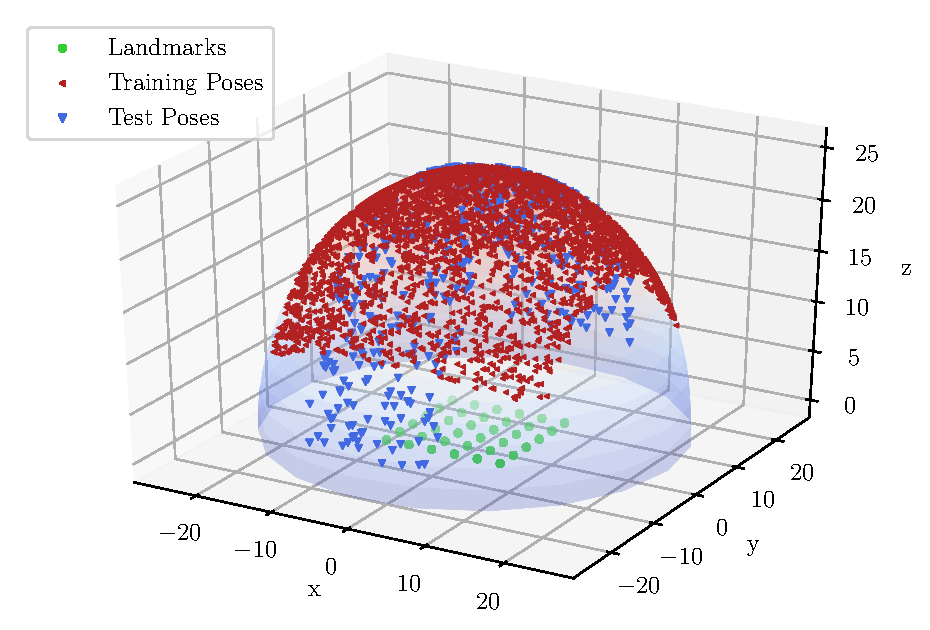
\includegraphics[width=0.5\textwidth]{probe-gk/sim_world.pdf}
   \label{fig:SimWorld} 
\caption{Our synthetic world. A stereo camera rig moves through a world with 2000 point features.}
\end{figure}

We simulated independent training and test traversals, where the camera moved for
30 and 60 seconds respectively (at a forward speed of 3 metres per second for final path
lengths of 90 and 180 meters).  \Cref{fig:sim_comparison} and \Cref{table:probe-gk_armse_errors} document the qualitative and quantitative comparisons of PROBE-GK (trained with and without ground-truth) against two baseline stereo odometry frameworks. Both baseline estimators were implemented based on \Cref{sec:ssvo}. The first utilized fixed covariances for all reprojection errors, while the second used a modified robust cost (i.e. M-estimation) based on Student's~$t$ weighting, with $\nu = 5$ (as suggested in \cite{kerl2013robust}).  These benchmarks served as baseline estimators (with and without robust costs) that used fixed covariance matrices and did not include a predictive component. 

Using PROBE-GK with ground truth data for training,
we significantly reduced both the translation and rotational Average Root Mean Squared Error (ARMSE)
by approximately 50\%. In our synthetic data, the Expectation Maximization approach was able to achieve nearly identical results to the ground-truth-aided model within 5 iterations.  

\begin{figure}
    \centering
    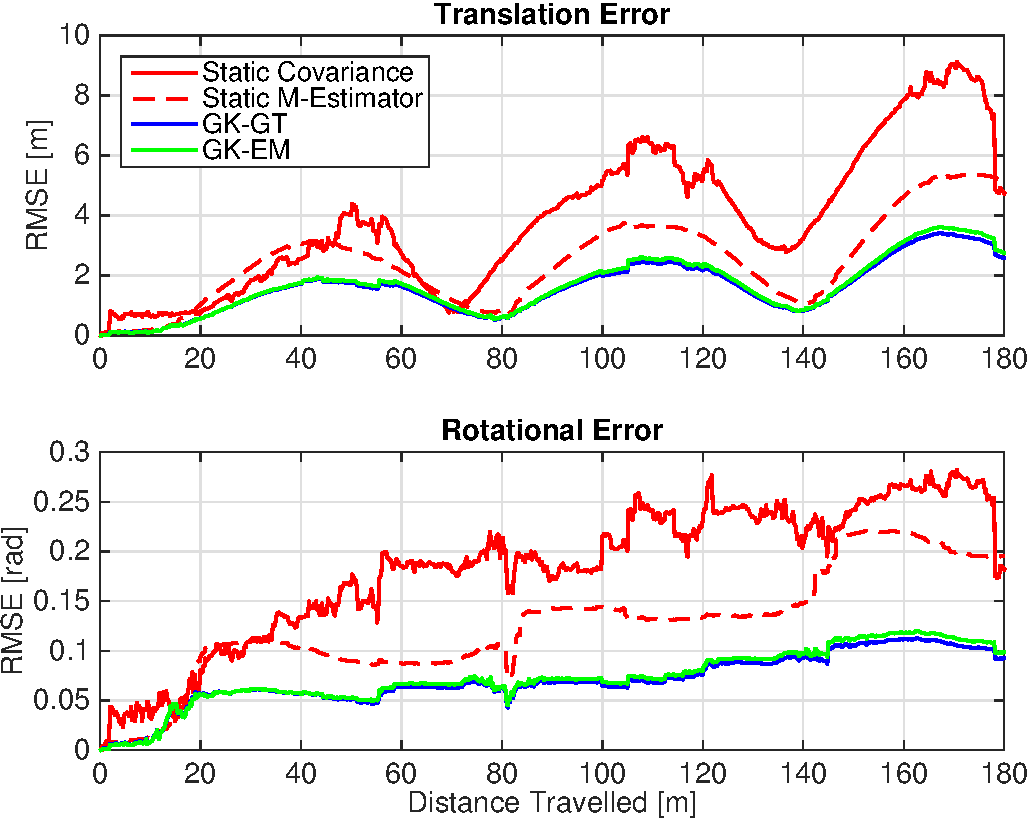
\includegraphics[width=0.75\textwidth]{probe-gk/simComparison_sim_rerun}
    \caption{A comparison of translational and rotational Root Mean Square Error on simulated data
    (RMSE) for four different stereo-visual odometry pipelines: two baseline
    bundle adjustment procedures with and without a robust Student's~$t$ cost with a fixed and
    hand-tuned covariance and degrees of freedom (M-Estimation), a robust bundle
    adjustment with covariances learned from ground truth with
    \cref{alg:train-ground-truth} (GK-GT), and a robust bundle adjustment using
    covariances learned without ground truth using expectation maximization,
    with \cref{alg:train-em} (GK-EM). Note in this experiment, the RMSE curves
    for GK-GT and GK-EM very nearly overlap. The overall translational and
    rotational ARMSE values are shown in Table \ref{table:probe-gk_armse_errors}.} 
    \label{fig:sim_comparison}
\end{figure}

\subsection{KITTI}

\begin{figure}
    \centering
    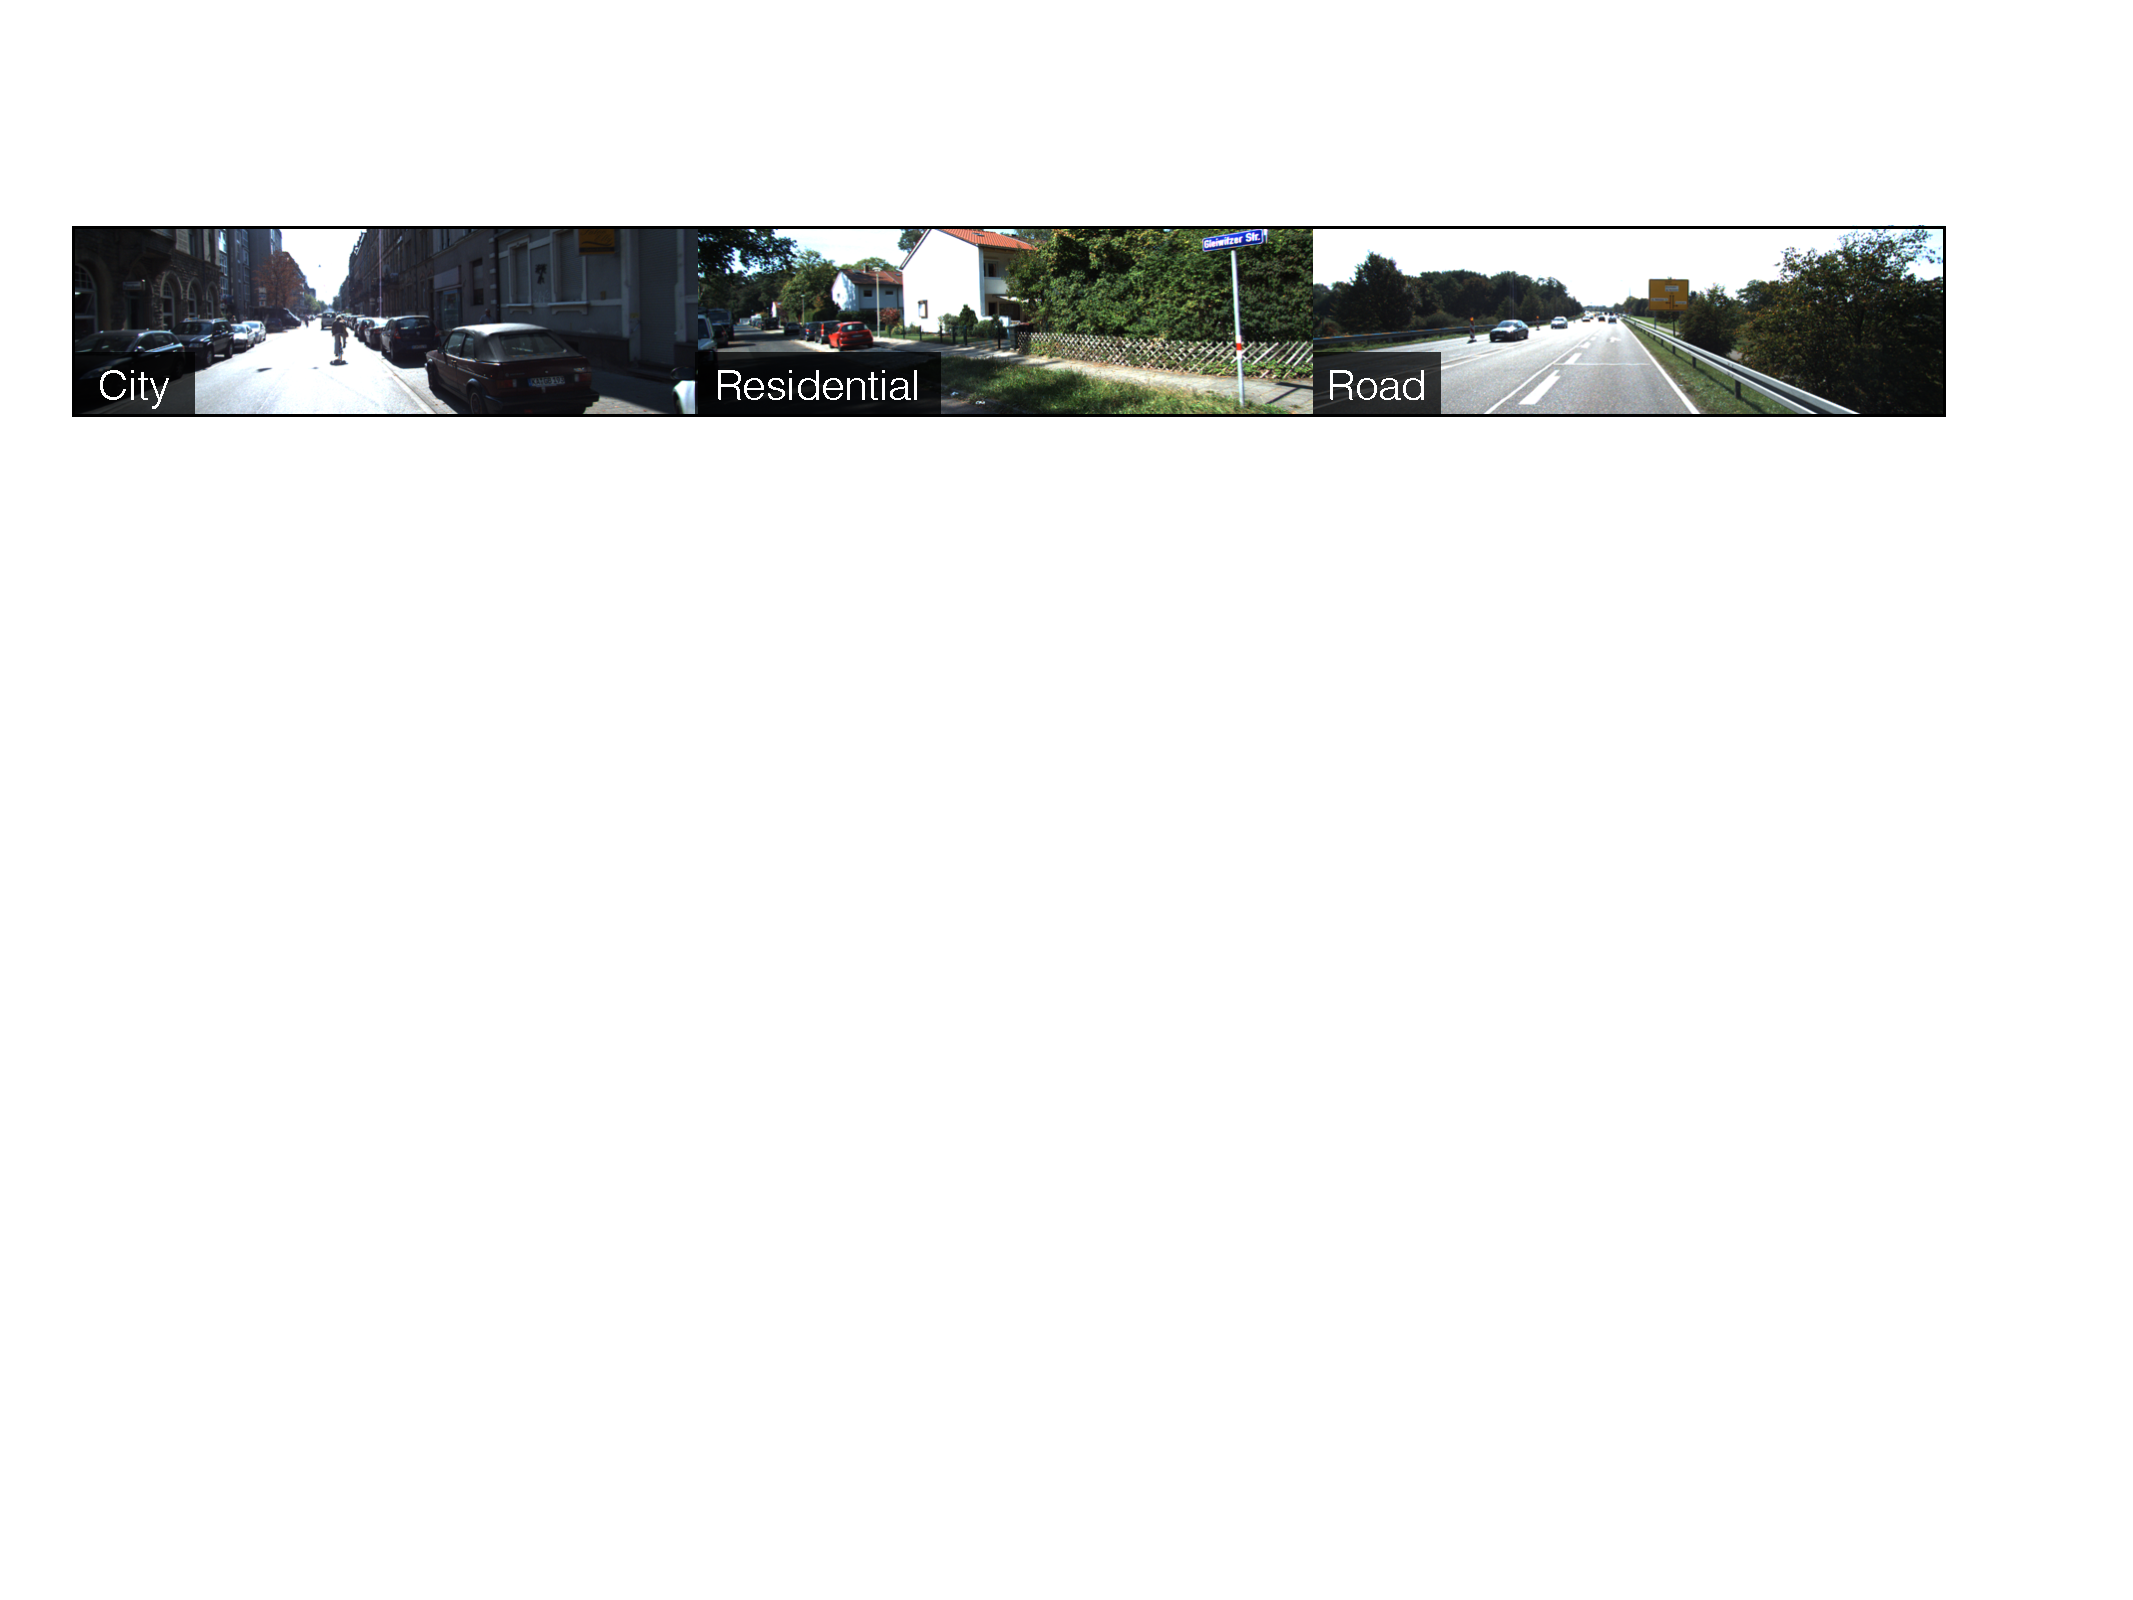
\includegraphics[width=0.98\textwidth]{probe-gk/KittiEnvironments}
    \caption{The KITTI dataset contains three different environments. We
      validate PROBE-GK by training on each type and testing against a baseline
      stereo visual odometry pipeline.}
      \vspace{-0.5em}
    \label{fig:kitti_environments}
\end{figure}

To evaluate PROBE-GK on real environments, we trained and tested several models on
the KITTI Vision Benchmark suite \citep{geiger2012kitti, geiger2013vision}, a series of datasets collected by a car outfitted with a number of
sensors driven around different parts of Karlsruhe, Germany. Within the dataset, ground truth pose information is
provided by a high grade inertial navigation unit which also fuses measurements from differential GPS. Raw data
is available for different types of environments through which the car was driving; for our
work, we focused on the city, residential and road categories
(\Cref{fig:kitti_environments}).  From each category, we chose two separate trials for training and testing.

\begin{figure}
    \centering
    \includegraphics[width=0.75\textwidth]{probe-gk/{kittiComparison-0011-0009-15-Sep-2015-4way}}
    \caption{RMSE comparison of stereo odometry estimators evaluated on data from the city category in the KITTI dataset. See \Cref{table:probe-gk_armse_errors} for a quantitative summary.}
    \vspace{-0.4em}
    \label{fig:probe-gk_kitti_comparison1}
\end{figure}

Our prediction space consisted  of inertial magnitudes, high and low image frequency
coefficients, image entropy, pixel location, and estimated transform parameters.
The choice of predictors is motivated by the types of effects we wish to capture
(in this case: grassy self-similar textures, as well as shadows, and motion blur). For
a more detailed explanation of our choice of prediction space, see our previous work
\citep{peretroukhin2015PROBE}.



\begin{figure}
    \centering
    \includegraphics[width=0.75\textwidth]{probe-gk/{kittiComparison-0035-0036-15-Sep-2015-4way}}
    \caption{RMSE comparison of stereo odometry estimators evaluated on data from the residential category in the KITTI dataset.}
    \vspace{-0.4em}
    \label{fig:probe-gk_kitti_comparison2}
\end{figure}

\begin{figure}
    \centering
    \includegraphics[width=0.75\textwidth]{probe-gk/{kittiComparison-0070-0028-15-Sep-2015-4way}}
    \caption{RMSE comparison of stereo odometry estimators evaluated on data from the road category in the KITTI dataset.}
    \vspace{-0.4em}
    \label{fig:probe-gk_kitti_comparison3}
\end{figure}

\Cref{fig:probe-gk_kitti_comparison1,fig:probe-gk_kitti_comparison2,fig:probe-gk_kitti_comparison3} show
typical results; \Cref{table:armse_errors} presents a quantitative comparison.
PROBE GK-GT produced significant reductions in ARMSE, reducing translational ARMSE by
as much as 80\%. In contrast, GK-EM showed more modest improvements; this is
unlike our synthetic experiments, where both GK-EM and GK-GT achieved similar
performance. We are still actively exploring why this is the case; we note that although our simulated
data is drawn from a mixture of Gaussian distributions, the underlying
noise distribution for real data may be far more complex. With no ground truth, EM has to jointly optimize the camera poses and sensor uncertainty. It is unclear whether this is feasible in the general case with no ground truth information.

Further, we observe that the performance of PROBE-GK depends on the similarity
of the training data to the final test trials. A characteristic training dataset was important for consistent improvements on test trials.





\subsubsection{UTIAS}

\begin{table}
\centering
\caption{Comparison of average root mean squared errors (ARMSE) for rotational
  and translational components. Each trial is trained and tested from a
  particular category of raw data from the synthetic and KITTI datasets.}

\resizebox{\columnwidth}{!}{%
\begin{tabular}{l c c c c c c c c c }
 & & \multicolumn{4}{c}{Trans. ARMSE [m]} & \multicolumn{4}{c}{Rot. ARMSE [rad]}  \\  \cline{3-6}  \cline{7-10} \T                                                                                    
 & Length [m] & Fixed Covar. & Static M-Estimator  & GK-GT & GK-EM & Fixed Covar. &  Static M-Estimator  & GK-GT & GK-EM  \\                         
\hline \T
Synthetic & 180 & 3.87 & 2.49 & 1.59 & 1.66 & 0.18 & 0.13 & 0.070 & 0.073 \\                                                                                                                
City & 332.9 & 3.84 & 2.99 & 1.69 & 2.87 & 0.032 & 0.021 & 0.0046 & 0.018 \\ 
Residential & 714.1 & 13.48 & 9.37 & 1.97 & 8.80 & 0.068 & 0.050 & 0.013 & 0.044 \\
Road & 723.8 & 17.69 & 9.38 & 5.24 & 8.87 & 0.060 & 0.027 & 0.015 & 0.024
\\ \hline                                                                                                                
\end{tabular}               \label{table:probe-gk_armse_errors}
}
\end{table}

\begin{figure}
    \centering
    \hspace*{0.25cm}
    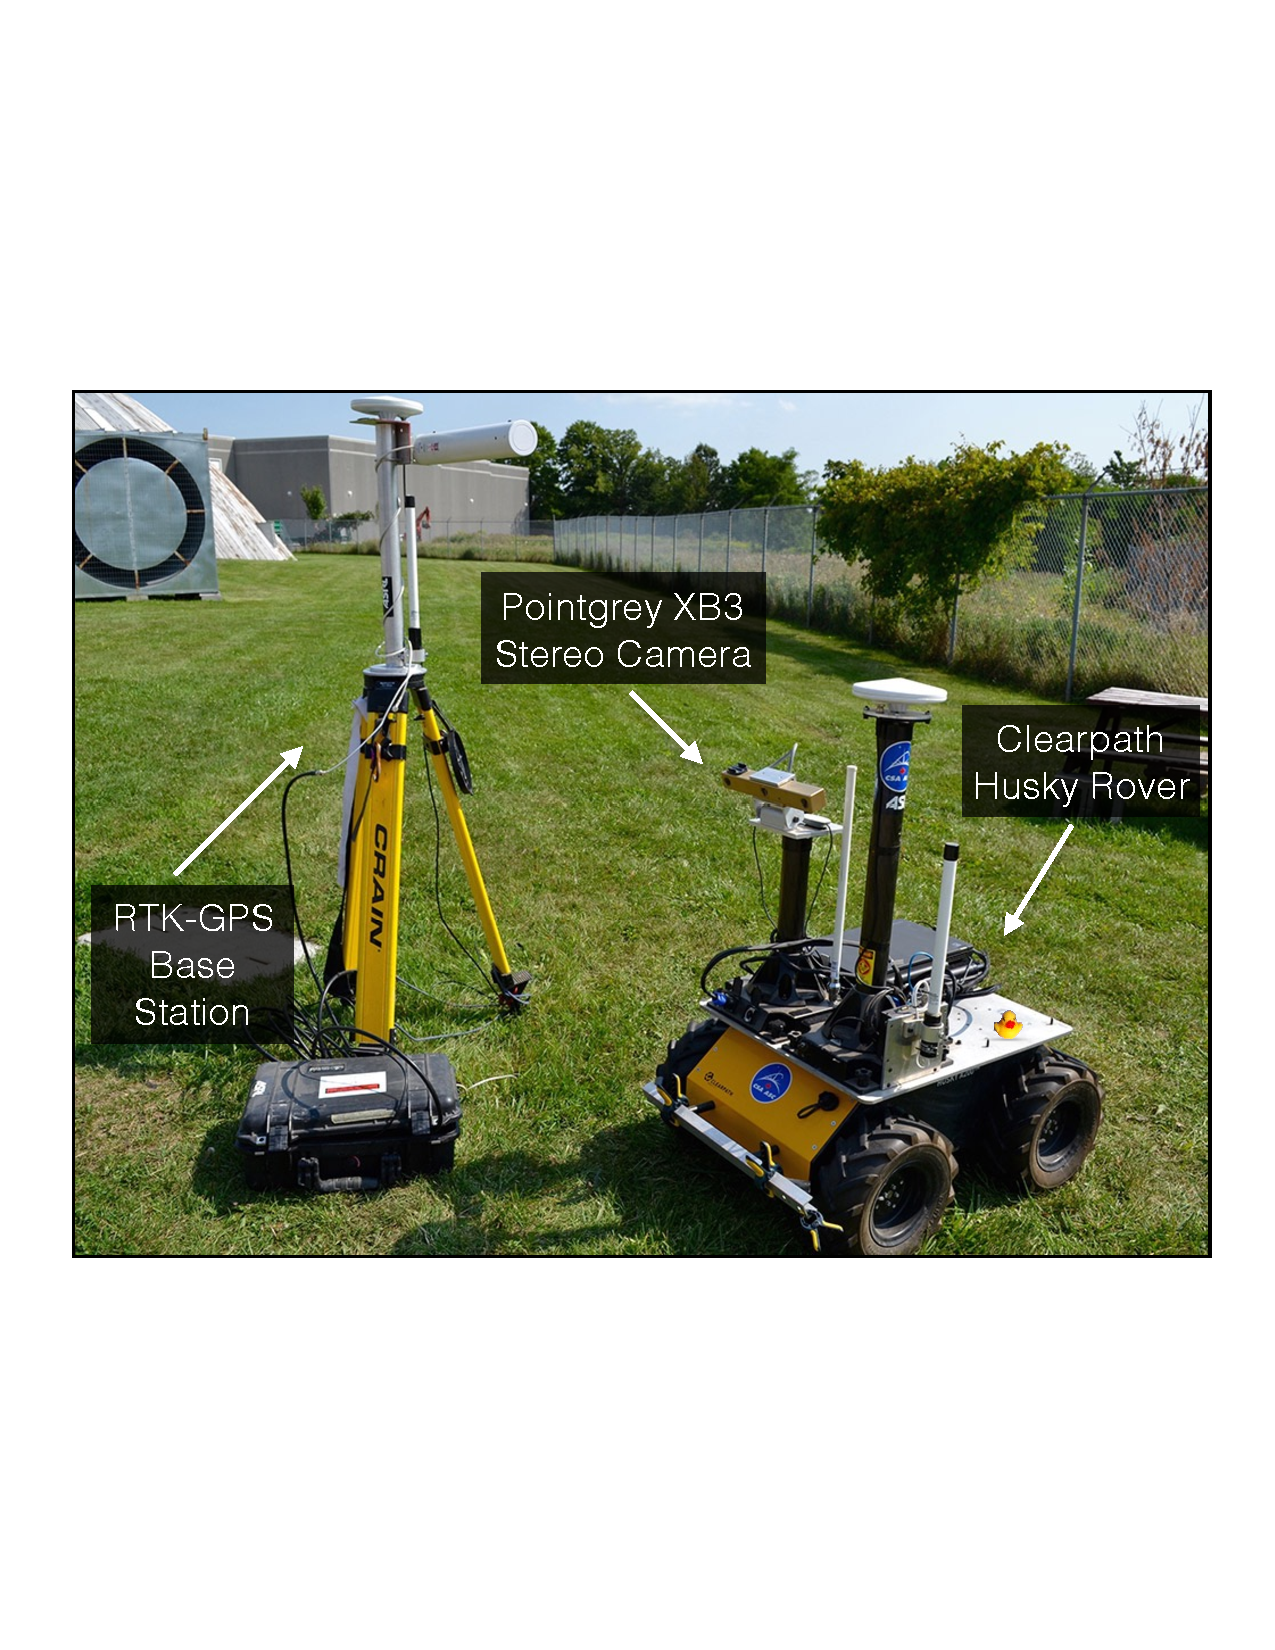
\includegraphics[width=0.75\textwidth]{probe-gk/experiment_wide_border}
    \caption{Our experimental apparatus: a Clearpath Husky rover outfitted with a PointGrey XB3 stereo camera and a differential GPS receiver and base station.}
      \vspace{-0.5em}
   	    \label{fig:probe-gk_experiments}
\end{figure}

\begin{figure}
    \centering
	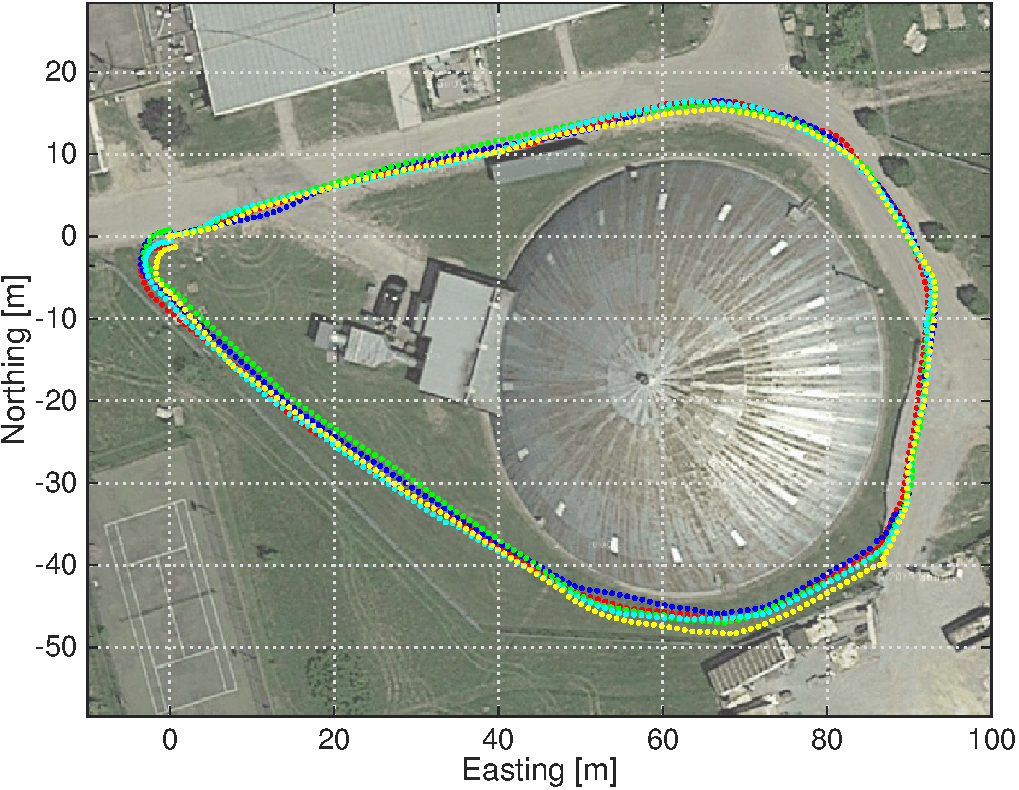
\includegraphics[width=0.75\textwidth]{probe-gk/xb3_rtk_fig}
    \caption{GPS ground truth for 5 experimental trials collected
      near the UTIAS Mars Dome. Each trial is approximately 250 m long.}
      \vspace{-0.5em}
    \label{fig:probe-gk_experiment_groundtruth}
\end{figure}

To further investigate the capability of our EM approach, we evaluated PROBE-GK on experimental data collected at the University of Toronto Institute for Aerospace Studies (UTIAS). For this experiment, we drove a Clearpath Husky rover outfitted with an Ashtech DG14 Differential GPS, and a PointGrey XB3 stereo camera around the MarsDome (an indoor Mars analog testing environment) at UTIAS (\Cref{fig:probe-gk_experiments}) for five trials of a similar path.  Each trial was approximately 250 m in length and we made an effort to align the start and end points of each loop. We used the wide baseline (25 cm) of the XB3 stereo camera to record the stereo images. The approximate trajectory for all 5 trials, as recorded by GPS, is shown in \Cref{fig:probe-gk_experiment_groundtruth}.  Note that the GPS data was not used during training, and only recorded for reference.

For the prediction space in our experiments, we mimicked the KITTI experiments, omitting inertial magnitudes as no inertial data was available. We trained PROBE-GK without ground truth, using the Expectation Maximization approach. \Cref{fig:probe-gk_experiments_trainingstats} shows the likelihood and loop closure error as a function of EM iteration. 

The EM approach indeed produced significant error reductions on the training dataset after just a few iterations.  Although  it was trained with no ground truth information, our PROBE-GK model was used to produce significant reductions in the loop closure errors of the remaining 4 test trials. This reinforced our earlier hypothesis: the EM method works well when the training trajectory more closely resembles the test trials (as was the case in this experiment). \Cref{table:probe-gk_loop_closure_errors} lists the statistics for each test. 


\begin{table}
\centering
\caption{Comparison of loop closure errors for 4 different experimental trials
  with and without a learned PROBE-GK-EM model.}
\begin{tabular}{ c  c  c  c }
     & & \multicolumn{2}{c}{Loop Closure Error [m]}  \\ \cline{3-4} \T
    Trial & Path Length [m] & PROBE-GK-EM & Static M-Estimator \\    
      \hline \T	
  2 & 250.3 & 3.88 & 8.07 \\
  3 & 250.5 & 3.07 & 6.64 \\
  4 & 205.4 & 2.81 & 7.57 \\
  5 & 249.9 & 2.34 & 7.75 \\ \hline
\end{tabular}
\label{table:probe-gk_loop_closure_errors}
\end{table}

\begin{figure}
    \centering
    \includegraphics[width=0.75\textwidth]{probe-gk/{trainingStats}}
    \caption{Training without ground truth using PROBE-GK-EM on a 250.2m path
      around the Mars Dome at UTIAS. The likelihood of the data increases with
      each iteration, and the loop closure error decreases, improving significantly from a baseline static M-estimator.}
      \vspace{-1em}
    \label{fig:probe-gk_experiments_trainingstats}
\end{figure}

\section{Summary}

Predictive Robust Estimation applied two different techniques (scalar weighted covariances and the method of generalized kernel estimation) to improve on the uncorrelated and static Gaussian error models typically employed in stereo odometry. PROBE and its follow up PROBE-GK, contributed
\begin{enumerate}
\item a probabilistic model for indirect stereo visual odometry, leading to a predictive robust algorithm for inference on that model,
\item two different approaches to constructing the robust algorithm: one based on k-nearest neighbours, and one based on Generalized Kernel (GK) estimation,
\item a procedure for training our model using pairs of stereo images with known relative transforms, and
\item an iterative, expectation-maximization approach to train our GK model when the relative ground truth egomotion was unavailable.
\end{enumerate}

%In this work, we presented PROBE, a novel method for predicting the quality of visual features within complex, dynamic environments. By using training data to learn a mapping from a predefined space of visual-inertial predictors to a scalar weight, we can adjust the influence of individual visual features on the final navigation estimate. PROBE can be used in place of traditional outlier rejection techniques such as RANSAC, or combined with them to more intelli- gently weight inlier measurements.
%We explored a variety of potential predictors, and validated our technique using a visual-inertial navigation system on over 4 km of data from the KITTI dataset and 700 m of indoor and outdoor data collected at the University of Toronto Institute for Aerospace Studies. Our results show that PROBE outperforms RANSAC-based binary outlier re- jection in many environments, even with only sparse ground truth available during the training step.
%In future work, we plan to examine a broader set of predic- tors, and extend the training procedure to incorporate online learning using intermittent ground truth measurements or loop closures detected by a place recognition thread. Further, we are interested in analyzing the amount of training data required for a given improvement in navigation accuracy, and in investigating PROBE’s effect on estimator consistency.


% By inferring a more accurate noise model given past sensory experience, we can reduce the tracking error of a sequence of estimates and improve the robustness of our estimator, even when the training data does not have associated ground truth. Our method has the advantage of having relatively few tuning parameters, meaning it can be applied to new problems with very little user intervention. We do rely on the availability of a good set of predictors, and have found that for problems of interest finding a good set is not difficult; a principled choice of an optimal set of predictors, however, remains an interesting open problem.
%Although our experiments demonstrate utility only in the context of sequential maximum likelihood estimation on stereo vision data, we believe the model presented here can be applied to a more general class of filter or factor- based estimation algorithms, as well as to a more general class of sensors. In future work, we plan to investigate the applicability of our method to problems of simultaneous localization and mapping, explore the possibility of learning the predictive model online (obviating the need for training data), and examine more principled approaches to selecting an informative prediction space.
